%---------------------------------------------------------------------%
%  LaTeX Course Notes Template                                        %
%                                                                     %
%  Copyright (C) 2012 Zev Chonoles                                    %
%  zevchonoles@gmail.com                                              %
%  http://math.uchicago.edu/~chonoles/                                %
%                                                                     %
%  Please leave this information in the source code as                %
%  attribution if you choose to edit or redistribute this file.       %
%                                                                     %
%  This work is licensed under the Creative Commons Attribution-      %
%  ShareAlike 3.0 Unported License. To view a copy of this license,   %
%  visit http://creativecommons.org/licenses/by-nc/3.0/.              %
%                                                                     %
%---------------------------------------------------------------------%

\documentclass[11pt]{article}






%----------%
%  Basics  %
%----------%


%  Specfies basic information.
%  In the metadata section of the preamble, you can specify the subject and a list of keywords for the PDF.
%
\newcommand{\coursetitle}{Measure Theory}
\newcommand{\lecturer}{Claudio Landim}
\newcommand{\notetaker}{Yao Zhang}
\newcommand{\notetakersemail}{jaafar\_zhang@163.com}
\newcommand{\courseterm}{Spring  2018}
\newcommand{\institution}{Instituto de Matem\'{a}tica Pura e Aplicada}


%  array provides more column styles for the tabular and array environments.
%  (http://ctan.org/pkg/array)
%
%  parskip sets block paragraphs as the default, instead of indentation.
%  (http://www.ctan.org/pkg/parskip)
%
\usepackage[margin=1in]{geometry}
\usepackage{amsmath,amssymb,amsthm,amsfonts,array,parskip}


%  Allows equation, align, gather, etc. environments to split across pages.
\allowdisplaybreaks


%  Sets date formatting to the ISO 8601 standard, YYYY-MM-DD.
\usepackage{datetime} \renewcommand{\dateseparator}{-} \yyyymmdddate






%---------%
%  Fonts  %
%---------%


%  Defines \cal for standard calligraphy, \eucal for Euler calligraphy, and \frak for Fraktur.
\usepackage{eucal}  \let\eucal\mathcal  \let\cal\CMcal  \renewcommand{\frak}{\mathfrak}


%  Removes ligatures (e.g. the connection ordinarily made between the two f's in "differentiable").
\usepackage{microtype} \DisableLigatures{encoding=*,family=*}
% 

%
\usepackage{scalerel,amssymb}
\def\mcirc{\mathbin{\scalerel*{\circ}{j}}}
\def\msquare{\mathord{\scalerel*{\Box}{gX}}}
% Arc (AB)
\DeclareSymbolFont{ugmL}{OMX}{mdugm}{m}{n}
\SetSymbolFont{ugmL}{bold}{OMX}{mdugm}{b}{n}
\DeclareMathAccent{\wideparen}{\mathord}{ugmL}{"F3}

%  Removes extra space after periods.
\frenchspacing






%-------------------------------%
%  Environments and Sectioning  %
%-------------------------------%


%  Defines some standard theorem environments, in both numbered and non-numbered versions. The numbering of every enviroment will be reset for each lecture.
\newcounter{lecture} \setcounter{lecture}{0}
%\newcounter{tN}[lecture]
%\newcounter{lN}[lecture]
        
\newtheorem{theorem}{Theorem}[lecture]              
\newtheorem{lemma}{Lemma}[lecture]      
\newtheorem{corollary}{Corollary}[lecture]  
\newtheorem{proposition}{Proposition}[lecture]
\theoremstyle{definition}    
\newtheorem{definition}{Definition}[lecture]          
\newtheorem{remark}{Remark}[lecture]      
\newtheorem{example}{Example}[lecture]
\newtheorem{comments}{Comments}[lecture]
\newtheorem{comment}{Comment}[lecture]
\newtheorem{warning}{Warning}[lecture]
\newtheorem{question}{Question}[lecture]
\newtheorem{exercise}{Exercise}[lecture]
\newtheorem{homework}{Homework}[lecture]
\newtheorem{notation}{Notation}[lecture]
\newtheorem{examples}{Examples}[lecture]
\newtheorem{claim}{Claim}[lecture]


%  Modifies the spacing above theorem environments, which is messed up when using the parskip package.
%  (http://tex.stackexchange.com/questions/22119)
%
\makeatletter \def\thm@space@setup{\thm@preskip=\parskip \thm@postskip=0pt} \makeatother


%  Modifies the spacing above the proof environment.
%  (http://tex.stackexchange.com/questions/49801)
%
\makeatletter \renewenvironment{proof}[1][\proofname]{\pushQED{\qed}\normalfont
\partopsep=\z@skip \topsep=\z@skip \trivlist \item[\hskip\labelsep\itshape #1\@addpunct{.}]
\ignorespaces}{\popQED\endtrivlist\@endpefalse} \makeatother


%  Removes extra space before and after section headings.
% \usepackage[compact]{titlesec}






%-------------------------%
%  Pictures and Diagrams  %
%-------------------------%


%  Allows for the use of colors.
%  (http://www.ctan.org/pkg/xcolor)
%
\usepackage[usenames,dvipsnames]{xcolor}
\definecolor{myred}{rgb}{0.9,0.2,0.2}
\definecolor{mygreen}{rgb}{0.2,0.6,0.2}
\definecolor{myblue}{rgb}{0.2,0.2,0.8}


%  graphicx provides advanced graphics options.
%  (http://ctan.org/pkg/graphicx)
%
\usepackage{subfig,graphicx,framed}
\graphicspath{ {img/} }


%  tikz is for drawing all sorts of pictures and diagrams.
%  tikz-cd makes creating commutative diagrams in tikz a bit easier.
%  (http://www.ctan.org/pkg/pgf)
%  (http://www.ctan.org/pkg/tikz-cd)
%
\usepackage{tikz}
\usepackage{tikz-cd}
\usetikzlibrary{arrows,calc,decorations,decorations.markings,fadings,positioning,patterns,shapes}
\tikzset{>=latex}
\tikzstyle{mypoint}=[inner sep=0pt,outer sep=0pt,minimum size=5pt,fill,circle]






%------------------------%
%  Commands and Symbols  %
%------------------------%


%  Creates commands by running over a comma-separated list. For example,
%
%     \forcsvlist{\define{\newcommand}{\textbf}{bold}}{A,B}
%
%  would create
%
%     \newcommand{\boldA}{\textbf{A}}    \newcommand{\boldB}{\textbf{B}}
%
%  (http://tex.stackexchange.com/a/5776/20882)
%
\usepackage{etoolbox}
\newcommand{\define}[4]{\expandafter#1\csname#3#4\endcsname{#2{#4}}}
\forcsvlist{\define{\DeclareMathOperator}{}{}}{im,coker,rad,nil,Ann,Ass,codim,Spec,mSpec,diam,ord,Supp,supp,disc,Ob,vol,rank,Sym,Alt,Ind}
\forcsvlist{\define{\newcommand}{\mathrm}{}}{Hom,Mor,id,GL,SL,SO,SU,U,M,Mat,Ext,Tor,Res,Cor,Inf,End,Irr,Aut,Gal,lcm,tr,sign,triv,diag,Map,op,ev,act,alg,sep,unr,nr,ab}

%  Creates commands for some names of categories in the sans-serif font.
\forcsvlist{\define{\newcommand}{\mathsf}{}}{Set,Grp,Ab,CRing,Mod,Vect,Cat,Top,PreSh,Sh,Sch,Nat,Fun,Diff}

%  Creates commands for some blackboard bold letters.
\forcsvlist{\define{\newcommand}{\mathbb}{}}{N,Z,Q,R,C,F,G,T,A,B,D}


%  Saves the section symbol, paragraph symbol, Hungarian accent, and Scandanavian O in the macros \SS, \PP, \HH, and \OO, then redefines \S, \P, \H, and \O to be the corresponding blackboard bold letters.
%
\let\SS\S  \let\PP\P  \let\HH\H  \let\OO\O
\forcsvlist{\define{\renewcommand}{\mathbb}{}}{S,P,H,O}


%  latexsym defines some alternative versions of amssymb symbols.
%  (http://www.bakoma-tex.com/doc/latex/base/latexsym.pdf)
%
\usepackage{latexsym}


%  Defines a copyright symbol that is a bit nicer than the built-in one.
\newcommand{\mycopyrightsymbol}{\raisebox{-0.3ex}{\tikz{\node[inner sep=0pt,outer sep=0pt] at (0,0) {\textsc{c}};\draw (0,0) circle (0.18);}}}


%  Defines commands for real and complex projective space.
\newcommand{\RP}{\mathbb{R}\mathrm{P}}  \newcommand{\CP}{\mathbb{C}\mathrm{P}}


%  Defines a bordered matrix with square bracket delimiters instead of parentheses.
%  (http://tex.stackexchange.com/questions/55054)
%
\let\bbordermatrix\bordermatrix
\patchcmd{\bbordermatrix}{8.75}{4.75}{}{}
\patchcmd{\bbordermatrix}{\left(}{\left[}{}{}
\patchcmd{\bbordermatrix}{\right)}{\right]}{}{}


%  Calls one of the mathabx font families so that it is possible to use its symbols without making a global change.
%  (http://www.ctan.org/pkg/mathabx)
%  (http://tex.stackexchange.com/questions/14386)
%
\DeclareFontFamily{U}{mathb}{\hyphenchar\font45}
\DeclareFontShape{U}{mathb}{m}{n}{<5> <6> <7> <8> <9> <10> gen * mathb
<10.95> mathb10 <12> <14.4> <17.28> <20.74> <24.88> mathb12}{}
\DeclareSymbolFont{mathb}{U}{mathb}{m}{n}


%  Defines circular arrows.
\DeclareMathSymbol{\lcirclearrow}{0}{mathb}{'366}
\DeclareMathSymbol{\rcirclearrow}{0}{mathb}{'367}
\newcommand{\leftcirclearrow}{\mathrel{\ensuremath{\raisebox{0.1ex}{\scalebox{0.9}{\rotatebox[origin=c]{90}{$\lcirclearrow$}}}}}}
\newcommand{\rightcirclearrow}{\mathrel{\ensuremath{\raisebox{0.1ex}{\scalebox{0.9}{\rotatebox[origin=c]{270}{$\rcirclearrow$}}}}}}


%  Gives semantic names for some common math symbols.
\newcommand{\iso}{\cong}
\newcommand{\htop}{\sim}
\newcommand{\htopequiv}{\simeq}
\newcommand{\cupprod}{\mathbin{\smallsmile}}
\newcommand{\capprod}{\mathbin{\smallfrown}}
\newcommand{\wedgesum}{\mathbin{\vee}}
\newcommand{\boundary}{\partial}
\renewcommand{\emptyset}{\varnothing}
\newcommand{\characteristic}{\mathrm{char}}
\newcommand{\symdiff}{\mathbin{\vartriangle}}
\newcommand{\convolute}{\mathbin{\ast}}
\newcommand{\actson}{\rightcirclearrow}
\newcommand{\actedonby}{\leftcirclearrow}
\newcommand{\directsum}{\oplus}
\newcommand{\bigdirectsum}{\bigoplus}
\newcommand{\tensor}{\otimes}
\newcommand{\bigtensor}{\bigotimes}
\newcommand{\free}{\mathbin{\ast}}
\newcommand{\bigfree}{\mathop{\ensuremath{\raisebox{-0.7ex}{\scalebox{2.3}{$\ast$}}}}}






%-----------------------------------%
%  Things Specific to Course Notes  %
%-----------------------------------%


%  Formatting for the table of contents. The first line allows for multi-column environments, the second line removes the heading "Contents".
\usepackage{multicol} \setlength{\columnsep}{3cm}
\makeatletter \renewcommand\tableofcontents{\@starttoc{toc}} \makeatother


%  Sets the page style.
\usepackage{fancyhdr}
\pagestyle{fancy}
\renewcommand{\headrulewidth}{0pt}
%\renewcommand{\footrulewidth}{0.5pt}
\setlength{\headheight}{14pt}
%\lfoot{\parbox[t]{1in}{\centering Last edited\\ \today}}
%\cfoot{\parbox[t]{3in}{\centering \coursetitle}}
%\rfoot{\parbox[t]{0.9in}{\centering Page \thepage\\ Lecture \arabic{lecture}}}


%  Sets the inputs for \maketitle.
\author{Lectures by \lecturer\\ \text{} \\ Notes by \notetaker}
\title{\coursetitle}
\date{\institution, \courseterm}


%  Defines headings for each day's notes.
\newcommand{\classheader}[1]{\stepcounter{lecture}\newpage\section*{ #1 } %\arabic{lecture}
\phantomsection \addcontentsline{toc}{section}{\arabic{lecture} #1}} %Lecture 


%---------------------------------------%
%  Miscellaneous Additions to Template  %
%---------------------------------------%

\newcommand{\ch}{\mathrm{ch}}
\newcommand{\pr}{\mathrm{pr}}
\newcommand\abs[1]{\lvert#1\rvert}
\newcommand{\Lie}{\mathrm{Lie}}
\newcommand{\Nil}{\mathrm{Nil}}
\newcommand{\spec}{\mathrm{spec}}
\usepackage[all]{xy}
\usepackage{stmaryrd}
\usepackage{mathtools}
\usepackage{pdfpages}  %jw -- needed to included a pdf page
\newcommand{\rcirclearrowleft}{\leftcirclearrow}
\newcommand{\lcirclearrowright}{\rightcirclearrow}

\usepackage{accents}
\newlength{\dhatheight}
\newcommand{\doublewidehat}[1]{%
    \settoheight{\dhatheight}{\ensuremath{\widehat{#1}}}%
    \addtolength{\dhatheight}{-0.35ex}%
    \widehat{\vphantom{\rule{1pt}{\dhatheight}}%
    \smash{\widehat{#1\, }}}\hspace{-0.03in}}
    
%\newlength{\dhatheight}
\newcommand{\doublewidetilde}[1]{%
    \settoheight{\dhatheight}{\ensuremath{\widetilde{#1}}}%
    \addtolength{\dhatheight}{-0.3ex}%
    \widetilde{\vphantom{\rule{1pt}{\dhatheight}}%
    \smash{\widetilde{#1\, }}}\hspace{-0.03in}}
    
%    \newlength{\dtildeheight}
    \newcommand{\doubleoverline}[1]{%
        \settoheight{\dhatheight}{\ensuremath{\overline{#1}}}%
        \addtolength{\dhatheight}{-0.35ex}%
        \widetilde{\vphantom{\rule{1pt}{\dhatheight}}%
        \smash{\overline{#1\, }}}\hspace{-0.03in}}


%---------------------------%
%  Hyperlinks and Metadata  %
%---------------------------%
%
% (this section must come last!)


%  hyperref enables for the creation of hyperlinks, and also specifies the metadata of the PDF file.
%  hyperxmp allows more metadata to be specified.
%  (http://www.ctan.org/pkg/hyperref)
%  (http://www.ctan.org/pkg/hyperxmp)
%  (http://tex.stackexchange.com/questions/41461)
%
\usepackage{hyperref}
\usepackage{hyperxmp}
\hypersetup{
pdfauthor={\notetaker},
pdftitle={\coursetitle},
pdfproducer={LaTeX},
pdfcopyright={Copyright (C) \the\year\ \notetaker. This work is licensed under a Creative Commons Attribution-ShareAlike 3.0 Unported License. All attribution should be to \lecturer\ as the lecturer, and to \notetaker\ as the person taking these notes.},
pdfsubject={},
pdfkeywords={},
pdflicenseurl={https://creativecommons.org/licenses/by-sa/3.0/},
colorlinks=true,
linkcolor=myred,
citecolor=mygreen,
urlcolor=myblue,
linktoc=page,
pdfstartview=FitH
}




\numberwithin{equation}{lecture}


%------------%
%  Document  %
%------------%


\begin{document}


%  The command
%
%  \thispagepdflabel{text}
%
%  sets the PDF page number (*not* the internal LaTeX page number) to be "text". This does not have to be a numeral; it could be a word, e.g. "Title". This lets one avoid the issue of having the PDF's page numbering not aligning with the page numbering LaTeX used in the document.
%
%  (http://tex.stackexchange.com/questions/85558)


%  Title
%
\maketitle
\thispdfpagelabel{Title}
\thispagestyle{empty}
\setcounter{page}{-1}
\vspace{0.3in}



%  Table of Contents
%
\begin{center}
\begin{minipage}[t]{0.9\textwidth}
\begin{multicols}{2}
\tableofcontents
\end{multicols}
\end{minipage}
\end{center}



\newpage
\thispdfpagelabel{-}
\thispagestyle{empty}



%  Introduction
%
\section*{Introduction}
These lectures are mainly based on the books Introduction to measure and integration by S. Taylor published by Cambridge University Press.

These notes were live-TeXed, though I edited for typos and added diagrams requiring the Ti\textit{k}Z package separately. I used the editor TeXstudio.

I am responsible for all faults in this document, mathematical or otherwise; any merits of the material here should be credited to the lecturer, not to me.

Please email any corrections or suggestions to \expandafter\href{mailto:\notetakersemail}{\texttt{\notetakersemail}}.

\medskip

\section*{Acknowledgments}

Thank you to all of my friends  who will send me suggestions and corrections. My notes will be  much improved due to your help.

I would like to especially thank the IMPA and Professor Landim  who put their courses in website.

\medskip

%  Copyright
%
%\section*{Copyright}
%Copyright \mycopyrightsymbol\ 2012 \notetaker.
%
%This work is licensed under a Creative Commons Attribution-ShareAlike 3.0 Unported License. This means you are welcome to do essentially anything with this work, including editing, adapting, distributing, and making commercial use of it, as long as you
%\begin{itemize}
%\item include an attribution of \lecturer\ as the lecturer of the course these notes are based on, and \notetaker\ as the person taking the notes,
%\item do so in a way that does not suggest either of us endorses you or your use of this work, and
%\item if you alter, transform, or build upon this work, you must apply to your work the same, or similar, license to this one.
%\end{itemize}
%More details are available at \href{https://creativecommons.org/licenses/by-sa/3.0/deed.en\_US}{\texttt{https://creativecommons.org/licenses/by-sa/3.0/deed.en\_US}}.

\newpage


%  Make a separate file for each lecture, for example, using a naming scheme like this:
%
%  lecture1.tex, lecture2.tex, ...
%
%  and keep them in the same folder as this main file. By doing it this way (instead of keeping all the notes in the main file), if you're only working on the notes for one lecture, you can easily comment out the lines corresponding to the other lectures.
%

\classheader{Lecture 1}
\setcounter{lecture}{1}

\begin{center}
	\Large \bf Introduction: a Non-measurable Set
\end{center}

\vspace{0.25cm}

$ \lambda $  satisfies the flowing: 
\begin{enumerate}
	\setcounter{enumi}{-1}
	\item $\lambda :\;\mathcal{P}\left( \mathbb{R} \right) \to {\mathbb{R}_ + } \cup \left\{ { + \infty } \right\}$
	\item $\lambda \left( {\left( {a,b} \right]} \right) = b - a$
	\item $A \subseteq \mathbb{R},\;A + x = \left\{ {x + y:\;y \in A} \right\},\;\;\forall A,\;A \subseteq \mathbb{R},\;\forall x \in \mathbb{R} : $
	\begin{equation}
	\lambda \left( {A + x} \right) = \lambda \left( A \right)
	\end{equation}
	\item $A = \bigcup\limits_{j \geqslant 1} {{A_j}} ,\;\;{A_j} \cap {A_k} = \emptyset : $
	\begin{equation}
	\lambda \left( A \right) = \sum\limits_k {\lambda \left( {{A_k}} \right)} 
	\end{equation}
\end{enumerate}


\begin{definition}
	$ x \sim y $,   $ x,y \in \mathbb{R} $ if $ y - x \in \mathbb{Q}. \left[ x \right] = \left\{ {y \in \mathbb{R},\;y - x \in \mathbb{Q}} \right\}. \\
	\text{} \qquad \qquad \qquad \quad  \ \ \Lambda  = \mathbb{R}{|_ \sim }$, only one point represents the equivalence class of $ \Omega $ , like $ \alpha, \beta.$
\end{definition}

$ \Omega $ is a class of equivalence class, if $\Omega  \subseteq R,\Omega  \subseteq \left( {0,1} \right)$

\begin{claim}
	$\left\{ \begin{matrix} 
	\Omega  + q = \Omega  + q \hfill \cr 
	\Omega  + q \cap \Omega  + q = \emptyset  \hfill \cr 
	\end{matrix}  \right.\;\;\;q,p \in \mathbb{Q}$
\end{claim}

\begin{proof}
	Assume that $ \Omega  + q \cap \Omega  + q \ne \emptyset $ then, $x = \alpha  + p = \beta  + q,\;\alpha ,\beta  \in \Omega \Rightarrow \alpha  - \beta  = q - p \in \mathbb{Q} \Rightarrow \alpha  = \beta  \Rightarrow \left[ {q \ne p,p,q \in \mathbb{Q} \Rightarrow \left( {\Omega  + q} \right) \cap \left( {\Omega  + p} \right) = \emptyset } \right].$
\end{proof}

\begin{claim}
	$\Omega  + q \subseteq \left( { - 1,2} \right)$, if  $ -1 < q < 1 $.
\end{claim}
 
then we can get 

\begin{equation}
\sum\limits_{\scriptstyle q \in \mathbb{Q} \hfill \atop 
	\scriptstyle  - 1 < q < 1 \hfill}  {\left( {\Omega  + q} \right)}  \subseteq \left( { - 1,2} \right)
\end{equation}

\begin{claim}
	$E \subseteq F \Rightarrow \lambda \left( E \right) \leqslant \lambda \left( F \right)$
\end{claim}
\begin{proof}
	$\because E \subseteq F\therefore F = E \cup \left( {F\backslash E} \right),\;E \cap \left( {F\backslash E} \right) = \emptyset $, then
	$\lambda \left( F \right) = \lambda \left( E \right) + \lambda \left( {\left( {F\backslash E} \right)} \right) \Rightarrow \lambda \left( F \right) \geqslant \lambda \left( E \right)$.
\end{proof}
Then,  
\begin{equation}
\lambda \left( {\sum\limits_{\scriptstyle q \in \mathbb{Q} \hfill \atop 
		\scriptstyle  - 1 < q < 1 \hfill}  {\left( {\Omega  + q} \right)} } \right) \leqslant \lambda \left( {\left( { - 1,2} \right)} \right) = 3
\end{equation}

and ,
\begin{equation}
\infty \cdot \lambda \left( {\left( {\Omega  + q} \right)} \right) =  \infty \cdot \lambda \left( \Omega  \right) \le 3 \Rightarrow \lambda \left( {\sum\limits_{\scriptstyle \;\;q \in \mathbb{Q} \hfill \atop 
		\scriptstyle  - 1 < q < 1 \hfill}  {\left( {\Omega  + q} \right)} } \right) = 0
\end{equation}

\begin{claim}
	$\left( {0,1} \right) \subseteq \sum\limits_{\scriptstyle \;\;q \in \mathbb{Q} \hfill \atop 
		\scriptstyle  - 1 < q < 1 \hfill}  {\left( {\Omega  + q} \right)} $
\end{claim}

\begin{proof}
	$ \forall $ fixed $  x \in \left( {0,1} \right), \exists \alpha  \in \left[ x \right] \cap \Omega ,\;\alpha  \in \left( {0,1} \right) $, and we know that $\alpha  - x = q \in \mathbb{Q},\; -  < q < 1\; \Rightarrow x = \alpha  + q,\;x \in \Omega  + q$
\end{proof}

But, we get that: 
\begin{equation}
1 = \lambda \left( {\left( {0,1} \right)} \right) \leqslant \lambda \left( {\sum\limits_{q \in \mathbb{Q}} {\Omega  + q} } \right) = 0
\end{equation}
it is impossible. 
\classheader{Lecture 2}
\setcounter{lecture}{2}

\begin{center}
	 \bf Classes of Subsets (Semi-algebras, Algebras and Sigma-algebras) and Set Functions
\end{center}

\vspace{0.25cm}
 
\begin{definition}
	$ \mathcal{S} \subseteq \mathcal{P} \left( \Omega  \right) $, $ \mathcal{S} $ is semi-algebra if:
	\begin{enumerate}
		\item $ \Omega \subseteq \mathcal{S} $
		\item $ A,B \in \mathcal{S} \Rightarrow A\bigcap B \in \mathcal{S} $
		\item $ \forall A \in \mathcal{S} \Rightarrow {A^c} = \sum\limits_{i = 1}^n {{E_j}} ,\;\;\exists {E_1}, \cdots ,{E_n} \in \mathcal{S} $, $ E_{i},E_{j} \left(i \ne j\right) $ disjoint sets, $ n $ is finite number
	\end{enumerate}
	\label{def2.1}
\end{definition}

\begin{example}
	$\Omega  = \mathbb{R},\;\mathcal{S} = \left\{ {\mathbb{R},\left\{ {\left( {a,b} \right),a < b,a,b \in \mathbb{R}} \right\},\left\{ {\left( { - \infty ,b} \right],b \in \mathbb{R}} \right\},\left\{ {\left( {a,\infty } \right),a \in \mathbb{R}} \right\},\emptyset } \right\}$, ${\left( {a,b} \right]^c} = \left( { - \infty ,a} \right] \cup \left[ {b, + \infty } \right)$
\end{example}

\begin{example}
	\small  
	$\Omega  = {{\mathbb R}^2}$
	
	${\mathcal S} = {\text{ }}\left\{ {{{\mathbb R}^2}} \right.,\left\{ {\left( {{a_1},{b_1}} \right) \times \left( {{a_2},{b_2}} \right),\;{a_i} < {b_i},{a_i},{b_i} \in {\mathbb R},\left\{ {\left( { - \infty ,{b_1}} \right] \times \left( { - \infty ,{b_2}} \right],{b_i} \in {\mathbb R}} \right\},\left\{ {\left( {{a_1},\infty } \right) \times \left( {{a_2},\infty } \right),{a_i} \in {\mathbb R}} \right\},\emptyset } \right\}$
\end{example}

\begin{definition}
	$ a = \mathcal{P}\left(\Omega\right) $ is an algebra:
	\begin{enumerate}
		\item $ \Omega  \in a$ 
		\item $ A,B\in a \Rightarrow A\bigcap B \in a  $
		\item $ A \in a \Rightarrow A^{c} \in a  $
	\end{enumerate}
\end{definition}

\begin{remark}
	$ a $ algebra $ \Rightarrow $ $ a $ semi-algebra
\end{remark}

\begin{definition}
	$ \sigma$-algebra $ \mathcal{S} \subseteq \mathcal{P}\left(\Omega\right) $:
	\begin{enumerate}
		\item $ \Omega \subseteq \mathcal{S} $
		\item $ A_{j} \in \mathcal{S}, j\le 1 \Rightarrow \bigcap\limits_{j \geqslant 1} {{A_j}}  \in \mathcal{S} $
		\item $ A \in \mathcal{S} \Rightarrow {A^c} \in \mathcal{S}$
	\end{enumerate}
\end{definition}

\begin{remark}
	$ \Omega, a_{\alpha} \subseteq \mathcal{P}\left(\Omega\right) $, $ a_{\alpha} $ algebra, $ \alpha \in I $ $ \Rightarrow a = \bigcap\limits_{\alpha  \in I} {{a_\alpha }} $ is an algebra.
\end{remark}

\begin{proof}
	check the followings
	\begin{enumerate}
		\item $ \Omega \in a  $
		\item $ A,B \in a \Rightarrow A \bigcap B \in a $
		\item $ A \in a \Rightarrow A^{c} \in a $
	\end{enumerate}
\end{proof}

\begin{remark}
	$ \Omega, a_{\alpha} \subseteq \mathcal{P}\left(\Omega\right), \alpha \in I, a_{\alpha} $, $ \sigma $-algebra $ \Rightarrow a = \bigcap\limits_{\alpha  \in I} {{a_\alpha }} $  is a $ \sigma $-algebra
\end{remark}

\begin{proof}
	check the followings
	\begin{enumerate}
		\item $ \Omega \in a  $
		\item $ A_{j}, j \ge 1 \in a \Rightarrow \bigcap\limits_{j \geqslant 1} {{A_j}}  \in a$
		\item $ A \in a \Rightarrow A^{c} \in a $
\end{enumerate}
\end{proof}

\begin{definition}[ minimal algebra generated by $ c $]
	$ \Omega, c \subseteq \mathcal{P}\left(\Omega\right) $, $ a \left(c\right) $ is an algebra generated by $ c $, and $ a = a\left(c\right) $:
	\begin{enumerate}
		\item $ c \subseteq a $ 
		\item $ \forall  \mathcal{B} $ is algebra, $ \mathcal{B} \subseteq \mathcal{P}\left(\Omega\right) $:
		\begin{equation}
		 c \subseteq \mathcal{B} \Rightarrow a \subseteq \mathcal{B} 
		\end{equation}
	\end{enumerate}
\end{definition}

\begin{remark}
	$ a\left(c\right) $ exits, and $a = a\left( c \right) = \bigcap\limits_\alpha  {{a_\alpha }} ,\;\forall \alpha ,\;c \subseteq {a_\alpha },\;{a_\alpha }$ is an algebra.
\end{remark}

\begin{definition}[ minimal $ \sigma $-algebra generated by $ c $]
	$ \Omega, c \subseteq \mathcal{P}\left(\Omega\right) $, $ a \left(c\right) $ is a $ \sigma $-algebra generated by $ c $, and $ a = a\left(c\right) $:
	\begin{enumerate}
		\item $ c \subseteq a $ 
		\item $ \forall  \mathcal{B} $ is $ \sigma $-algebra, $ \mathcal{B} \subseteq \mathcal{P}\left(\Omega\right) $:
		\begin{equation}
		c \subseteq \mathcal{B} \Rightarrow a \subseteq \mathcal{B} 
		\end{equation}
	\end{enumerate}
\label{def2.5}
\end{definition}

\begin{remark}
	$ a\left(c\right) $ exits, and $a = a\left( c \right) = \bigcap\limits_\alpha  {{a_\alpha }} ,\;\forall \alpha ,\;c \subseteq {a_\alpha },\;{a_\alpha }$ is an $ \sigma $-algebra.
	\label{rmk2.5}
\end{remark}

\begin{lemma}
	$ \Omega, f $ semi-algebra $ f \subseteq \mathcal{P}\left(\Omega\right) $, $ a\left(f\right) $ algebra generated by $ f $ then 
	\begin{equation}
	A \in a\left(f\right) \Leftrightarrow \exists {E_j} \in f,1 \leqslant j \leqslant n,\;A = \sum\limits_{j = 1}^n {{E_j}} 
	\end{equation}
	\label{lma2.1}
\end{lemma}

\begin{proof}
	\text{}
	\begin{enumerate}
		\item $ \Leftarrow $ 
		
		$A = \sum\limits_{j = 1}^n {{E_j}} , \ {E_j} \in f \in a \left(f\right)$
		
		By definition \ref{def2.1} and remark \ref{rmk2.6} $ \Rightarrow A \in a \left(f\right) $
		\item $ \Rightarrow $
		
		$ A \in a\left(f\right) \Rightarrow A = \sum\limits_{j = 1}^n {{E_j}} ,{E_j} \in f $
		
		Then by remark \ref{rmk2.7}, it will be  proved easily.
	\end{enumerate}
\end{proof}

\begin{remark}
	$ E,J \in a, E \bigcup F \in a, E \bigcup F= \left(E^{c} \bigcap F^{c}\right)^{c} $
	\label{rmk2.6}
\end{remark}

\begin{remark}
	$ \mathcal{B} =\left\{ {\sum\limits_{j = 1}^n {{F_j},\;{F_j} \in f} } \right\},\;\mathcal{B} \subseteq \mathcal{P}\left( \Omega  \right) $ then
	\begin{enumerate}
		\item $ \mathcal{B} $ algebra
		\item $ \mathcal{B} \supseteq f $
		\item $ \mathcal{B} \supseteq a\left(f\right) $
	\end{enumerate} 
	\label{rmk2.7}
\end{remark}

\begin{proof}
	We only prove that  $ \mathcal{B} $ algebra, then check the following
	\begin{enumerate}
		\item $ \Omega \in \mathcal{B} $
		\item $A,B \in \mathcal{B} \Rightarrow A \cap B \in \mathcal{B}$
		
		$ \because A,B \in \mathcal{B}, $ $ \therefore A = \sum\limits_{j = 1}^n {{E_j}} ,\;{E_j} \in f,\;B = \sum\limits_{k = 1}^m {{F_k}} ,\;{F_k} \in f$, then 
		\begin{equation}
		\begin{split}
		A \cap B & = \left( {\sum\limits_{j = 1}^n {{E_j}} } \right) \cap \left( {\sum\limits_{k = 1}^m {{F_k}} } \right)\\
				 & = \sum\limits_{j = 1}^n {\sum\limits_{k = 1}^m {\underbrace {\left( {{E_j} \cap {F_k}} \right)}_{ \in f}} } \\
				 & \in  \mathcal{B}
		\end{split}
		\end{equation}
		
		\item $ A \in \mathcal{B} \Rightarrow A^{c} \in \mathcal{B} $
		
		$A = \sum\limits_{j = 1}^n {{E_j}} ,\;{E_j} \in f$ 
		
		By definition \ref{def2.1}:
		\begin{equation}
		\begin{split}
		E_1^c  & = \sum\limits_{{k_1} = 1}^{{l_1}} {{F_{1,{k_1}}}} ,\;{F_{1,j}} \in f \\
		\cdots & =  \cdots \\
		E_i^c & = \sum\limits_{{k_i} = 1}^{{l_i}} {{F_{i,{k_i}}}} ,\;{F_{i,j}} \in f
		\end{split}
		\end{equation}
		
		Then, we get that 
		\begin{equation}
		\begin{split}
		{A^c} & = \left( {\sum\limits_{{k_1} = 1}^{{l_1}} {{F_{1,{k_1}}}} } \right) \cap \left( {\sum\limits_{{k_2} = 1}^{{l_2}} {{F_{2,{k_2}}}} } \right) \cap  \cdots  \cap \left( {\sum\limits_{{k_n} = 1}^{{l_n}} {{F_{n,{k_n}}}} } \right)\\
		      &  = \sum\limits_{{k_1} = 1}^{{l_1}} {\sum\limits_{{k_2} = 1}^{{l_2}} { \cdots \sum\limits_{{k_n} = 1}^{{l_n}} {\left( {{F_{1,{k_1}}} \cap {F_{2,{k_2}}} \cap {F_{n,{k_n}}}} \right)} } } \\
		      & \in \mathcal{B}
		\end{split}
		\end{equation}
	\end{enumerate}
\end{proof}

\begin{definition}
	$ c \subseteq\mathcal{P}\left(\Omega\right), \emptyset \in c $, $\mu :\;c \to {\mathbb{R}_ + } \cup \left\{ { + \infty } \right\}$. $ \mu $ is additive if 
	\begin{enumerate}
		\item $\mu \left( \emptyset  \right) = 0$
		\item ${E_1},{E_2},...,{E_n} \in c,\;E = \sum\limits_{j = 1}^n {{E_j}}  \in c \Rightarrow \mu \left( E \right) = \sum\limits_{j = 1}^n {\mu \left( {{E_k}} \right)} $
	\end{enumerate}
	\label{def2.6}
\end{definition}

\begin{remark}
	\begin{equation}
	\exists A \in c,\;\mu \left( A \right) < \infty ,\;A = A \cup \emptyset ,\;\mu \left( A \right) = \mu \left( A \right) + \mu \left( \emptyset  \right) \Rightarrow \mu \left( \emptyset  \right) = 0
	\label{eq2.7}
	\end{equation}
	\label{rmk2.8}
\end{remark}

\begin{remark}
	$ c,\  \mu: c \to \mathbb{R}_{+} \bigcup {+ \infty}, \  E \subseteq F, \ F\backslash E \in c,\;E,F \in c $
	\begin{equation}
	F = E \cup \left( {F\backslash E} \right),\;\mu \left( F \right) = \mu \left( E \right) + \left( {F\backslash E} \right)
	\label{eq2.8}
	\end{equation}
	\begin{enumerate}
		\item $\mu \left( E \right) =  + \infty $, $\mu \left( F \right) =  + \infty $
		\item $\mu \left( E \right) <  + \infty $, $\mu \left( {F\backslash E} \right) = \mu \left( F \right) - \mu \left( E \right)$
	\end{enumerate}
	so, 
	\begin{equation}
	\mu \left( E \right) \leqslant \mu \left( F \right)
	\label{eq2.9}
	\end{equation}
	\label{rmk2.9}
\end{remark}

\begin{example}
	Discrete measure:
	$ \Omega $, $ c \subseteq  \mathcal{P}\left(\Omega\right) $, $\left\{ {{x_j},\;j \geqslant 1} \right\},\;{x_j} \in \Omega ,\;\left\{ {{p_j},\;j \geqslant 1} \right\},\;{p_j},  \geqslant 0$, $ A \in c, $ define that
	\begin{equation}
	\mu \left( A \right) = \sum\limits_{j \geqslant 1} {{p_j}} 1\left\{ {{x_j} \in A} \right\}
	\end{equation}
	then $ \mu $ is additive
	\label{eg2.3}
\end{example}

\begin{definition}
	$ c \in \mathcal{P}\left(\Omega\right), \emptyset \in c, $ $ \mu: \  c \to \mathbb{R}_{+} \bigcup {+ \infty }$, $ \mu $ is $ \sigma $-additive if  
	\begin{enumerate}
		\item $\mu \left( \emptyset  \right) = 0$
		\item ${E_j}\in c, \ j \ne k, E_{j} \bigcap E_{k} = \emptyset,\ \;E = \sum\limits_{j \ge  1} {{E_j}}  \in c \Rightarrow \mu \left( E \right) = \sum\limits_{j \ge 1} {\mu \left( {{E_j}} \right)} $
	\end{enumerate}
\end{definition}

\begin{example}
	$\Omega  = \left( {0,1} \right),\;c = \left\{ {\left( {a,b} \right],\;0 \leqslant a < b < 1} \right\},$ $\mu :\;c \to {\mathbb{R}_ + } \cup \left\{ { + \infty } \right\}$,  define that
	\begin{equation}
	\mu \left( {a,b} \right] = \left\{ {\begin{matrix}
		{ + \infty }  \\ 
		{b - a}  \\ 	
		\end{matrix} } \right.\;\;\begin{matrix}
	{a = 0}  \\ 
	{a > 0}  \\ 
	\end{matrix} 
	\end{equation}
	$\left( {a,b} \right] = \sum\limits_{j = 1}^n {\left( {{a_j},{b_j}} \right)} $,  we can get that  $ \mu $ is NOT $ \sigma $-additive.
	
	If  $ {x_1} = \frac{1}{2},{x_j} > {x_{j + 1}},{x_j} \downarrow  \to 0 $, then 
	\begin{equation}
	\frac{1}{2} = \left( {0,\frac{1}{2}} \right] = \sum\limits_{j \geqslant 1} {\left( {{x_{j + 1}},{x_j}} \right]}  =  + \infty 
	\end{equation}
	it is impossible.
\end{example}


\classheader{Lecture 3}
\setcounter{lecture}{3}

\begin{center}
	\Large \bf Set Functions
\end{center}

\vspace{0.25cm}

\begin{definition}
	$ c \subseteq \mathcal{P}\left(\Omega\right) $, $ \mu:  c \to \mathbb{R}_{+} \bigcup {+ \infty} $:
	\begin{enumerate}
		\item \label{def3.1.1} $ E \in c $, $ \mu $ continuous from below at $ E $, if $\forall {\left( {{E_n}} \right)_{n \geqslant 1}},\;{E_n} \in c,\;{E_n} \uparrow E\;\left( {{E_n} \subseteq {E_{n + 1}},\;\bigcup\limits_{n \geqslant 1} {{E_n} = E} } \right):$
		\begin{equation}
		\mu \left( {{E_n}} \right) \to \mu \left( E \right)
		\label{eq3.1}
		\end{equation}
		\item \label{def3.1.2}  $ E \in c $, $ \mu $ continuous from above at $ E $, if $\forall {\left( {{E_n}} \right)_{n \geqslant 1}},\;{E_n} \in c,\;{E_n} \downarrow E\;\left( {{E_{+1}} \subseteq {E_{n}},\;\bigcap\limits_{n \geqslant 1} {{E_n} = E} } \right),$ and $\exists {n_0},\;\mu \left( {{E_{{n_0}}}} \right) < \infty $:
		\begin{equation}
		\mu \left( {{E_n}} \right) \to \mu \left( E \right)
		\label{eq3.2}
		\end{equation}
	\end{enumerate}
\label{def3.1}
\end{definition}

\begin{remark}
	For a sequence $ E_{1},E_{2}, ... $ of sets, we put 
	\begin{equation}
	\lim \sup {E_i} = \bigcap\limits_{n = 1}^\infty  {\left( {\bigcup\limits_{i = n}^\infty  {{E_i}} } \right)} ,\lim \inf {E_i} = \bigcup\limits_{n = 1}^\infty  {\left( {\bigcap\limits_{i = n}^\infty  {{E_i}} } \right)} 
	\end{equation}
	and if $\left\{ {{E_i}} \right\}$ is such that ${\lim \sup E = \lim \inf {E_i}}$ we say that the sequence converges to the set 
	\begin{equation}
	{E = \lim \sup E = \lim \inf {E_i}}
	\end{equation}
	\label{rmk3.1}
\end{remark}

\begin{remark}
	\ref{def3.1.2} need $\exists {n_0},\;\mu \left( {{E_{{n_0}}}} \right) < \infty $, if not: \
	\begin{equation}
	{E_n} = \left[ {n, + \infty } \right),\;\mu \left( {{E_n}} \right) =  + \infty ,\;{E_n} \downarrow \emptyset ,\;\lambda \left( \emptyset  \right) = 0
	\label{eq3.3}
	\end{equation}
	\label{rmk3.2}
\end{remark}

\begin{lemma}
	$ a \subseteq \mathcal{P}\left(\Omega\right) $, algebra; $\mu :\;a \to {\mathbb{R}_ + } \cup \left\{ { + \infty } \right\}$, additive;
	\begin{enumerate}
		\item \label{lem3.1.1} $ \mu $ is $ \sigma $-additive $ \Rightarrow $ $ \mu  $ continuous at E, $ \forall E \in a $
		\item \label{lem3.1.2} $ \mu $ is continuous from below $ \Rightarrow $ $ \mu  $  is $ \sigma $-additive 
		\item \label{lem3.1.3} $ \mu $ is continuous from above at $ \emptyset \&  $ $ \mu $ is finite $ \Rightarrow $ $ \sigma $-additive 
	\end{enumerate}
\label{lem3.1}
\end{lemma}

\begin{proof}
	\text{}
	\begin{enumerate}
		\item \text{}
		
		(i) $ \mu  $ is $ \sigma $-additive $ \Rightarrow $ $ \mu $ conti. from below at $  E \in a. $
		\begin{figure}[!htb]
			\centering
			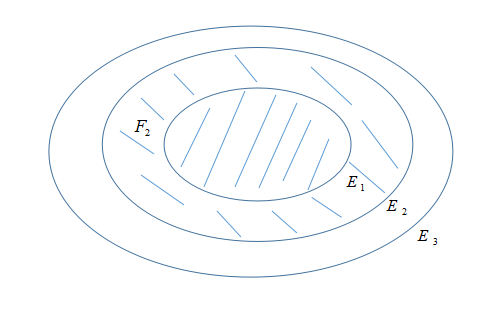
\includegraphics[width=0.3\linewidth,height=0.2\linewidth]{fig31.png}
			\label{fig31}
			%\caption{ illustration for $ 3 $}
		\end{figure}
	    $ E \in a, {E_n} \uparrow E,\;{E_n} \in a$:
	    \begin{equation}
	    \begin{split}
	    {F_1} & = {E_1} \\
	    {F_2} & = {E_2}\backslash {E_1}\\
	     \vdots \ \  & = \ \  \vdots  \\
	    {F_n} & = {E_n}\backslash {E_{n - 1}}
	    \end{split}
	    \label{eq3.4}
	    \end{equation}
	    and we can get that
	    \begin{equation}
	    {F_j} \cap {F_k} = \emptyset ,\quad \sum\limits_{k = 1}^n {{F_k}}  = {E_n}, \quad \bigcup\limits_{n \geqslant 1} {{E_n}}  = \bigcup\limits_{n \geqslant 1} {{F_n}} 
	    \label{eq3.5}
	    \end{equation}
	    so 
	    \begin{equation}
	    \mu \left( E \right) = \sum\limits_{k \geqslant 1} {\mu \left( {{F_k}} \right)}  = \mathop {\lim }\limits_{n \to \infty } \sum\limits_{k = 1}^n {\mu \left( {{F_k}} \right)}  = \mathop {\lim }\limits_{n \to \infty } \mu \left( {{E_n}} \right)
	    \label{eq3.6}
	    \end{equation}
		(ii) $ \mu $ cont. from above $ E \in a, {E_n} \in a,{E_n} \downarrow E,\mu \left( {{E_{{n_0}}}} \right) < \infty  \Rightarrow \mu \left( {{E_n}} \right) \downarrow \mu \left( E \right)$
		\begin{figure}[!htb]
			\centering
			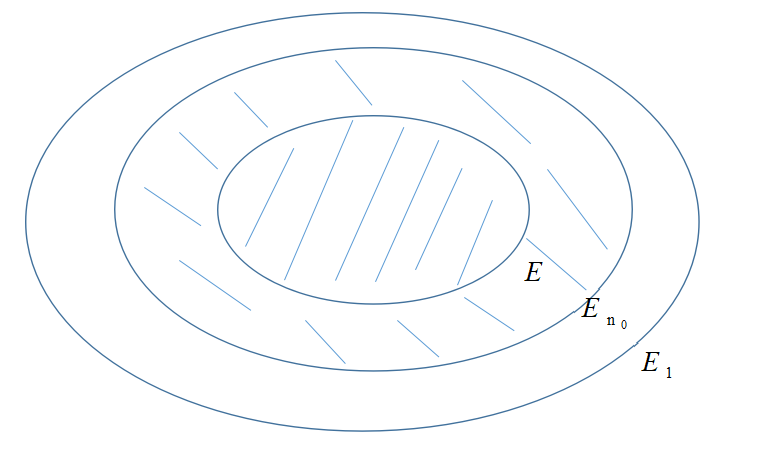
\includegraphics[width=0.3\linewidth,height=0.2\linewidth]{fig32.png}
			\label{fig32}
			%\caption{ illustration for $ 3 $}
		\end{figure}
		\begin{equation}
		\begin{split}
		{G_1} & = {E_{{n_0}}}\backslash {E_{{n_0} + 1}}\\
		{G_2} & = {E_{{n_0}}}\backslash {E_{{n_0} + 2}} \\
		\vdots \quad & = \quad \vdots\\
		{G_k} & = {E_{{n_0}}}\backslash {E_{{n_0} + k}}
		\end{split}
		\label{eq3.7}
		\end{equation}
		then ${G_k} \uparrow {E_{{n_0}}}\backslash {E}, {G_k} \in a \Rightarrow \mu \left( {{G_k}} \right) \uparrow \mu \left( {{E_{{n_0}}}\backslash E} \right)$, so
		
		\begin{equation}
		\begin{split}
		\mu \left( {{E_{{n_0}}}\backslash E} \right) & = \mathop {\lim }\limits_{n \to \infty } \mu \left( {{E_{{n_0}}}\backslash {E_{{n_0} + k}}} \right)\\
		\mu \left( {{E_{{n_0}}}\backslash E} \right) & = \mu \left( {{E_{{n_0}}}} \right) - \mu \left( E \right)\\
		\mu \left( {{E_{{n_0}}}} \right) - \mu \left( E \right) & = \mathop {\lim }\limits_{k \to \infty } \left( {\mu \left( {{E_{{n_0}}}} \right) - \mu \left( {{E_{{n_0} + k}}} \right)} \right)
		\end{split}
		\end{equation}
		\label{eq3.8}
		\item $ \mu $ cont. below, $E = \sum\limits_{k \geqslant 1} {{E_k}} ,\;E,{E_k} \in a$.
		
		Obs.
		\begin{equation}
		\sum\limits_{k = 1}^n {{E_k}}  \subseteq E \stackrel{additive}{\Rightarrow} \left\{ \begin{matrix} 
		\mu \left( {\sum\limits_{k = 1}^n {{E_k}} } \right) \leqslant \mu \left( E \right) \hfill \cr 
		\sum\limits_{k = 1}^n {\mu \left( {{E_k}} \right) \leqslant \mu \left( E \right)}  \hfill \cr 
		\end{matrix}  \right.
		\label{eq3.9}
		\end{equation}
		then
		\begin{equation}
		\sum\limits_{k \geqslant 1} {\mu \left( {{E_k}} \right)}  \leqslant \mu \left( E \right)
		\label{eq3.10}
		\end{equation}
		${F_n} = \sum\limits_{k = 1}^n {{E_k}}  \in a,\;{F_n} \uparrow E$, 
		\begin{equation}
		\sum\limits_{k = 1}^n {\mu \left( {{E_k}} \right)}  = \mu \left( {{F_n}} \right) \uparrow \mu \left( E \right) \Rightarrow \sum\limits_{k \geqslant 1} {\mu \left( {{E_k}} \right)}  = \mu \left( E \right)
		\label{eq3.11}
		\end{equation}
		\item $ \mu $ cont. at $ \emptyset $, $ \mu\left(\Omega\right) < \infty $, $ E,E_{k} \in a, E = \sum\limits_{k \geqslant 1} {{E_k}}. $ 
		\begin{equation}
		{F_n} = \sum\limits_{k \geqslant m} {{E_k}}  \in a\;\left( {E\backslash \sum\limits_{j = 1}^{n - 1} {{E_j}} } \right)
		\label{eq3.12}
		\end{equation}
		${F_n} \downarrow \emptyset ,\mu \left( {{F_1}} \right) < \infty ,\;\mu \left( {{F_n}} \right) \to 0$
		\begin{equation}
		\begin{split}
		\mu \left( E \right) & = \mu \left( {\sum\limits_{k = 1}^n {{E_k} \cup \sum\limits_{k > n} {{E_k}} } } \right)\\
							 & =  \underbrace {\mu \sum\limits_{k = 1}^n {{E_k}  } }_{ \to \sum\limits_{k \geqslant 1} {\mu \left( {{E_n}} \right)} } \ + \ \underbrace {\mu \sum\limits_{k > n} {{E_k}} }_{ \to 0}\\
							 & \to \sum\limits_{k \geqslant 1} {\mu \left( {{E_n}} \right)} 
		\end{split}
		\end{equation}
		\label{eq3.13}
	\end{enumerate}
\end{proof}

\begin{remark}
	Suppose ${E_\alpha },\;\alpha  \in I$ is a class of subsets of $ X $, and $ E_{i} $ is one set of the class, then
	\begin{enumerate}
		\item $\bigcap\limits_{\alpha  \in I} {{E_\alpha } \subseteq {E_i}}  \subseteq \bigcup\limits_{\alpha  \in I} {{E_\alpha }} $
		\item \label{rmk332}$ X - \bigcup\limits_{\alpha  \in I} {{E_\alpha }}  = \bigcap\limits_{\alpha  \in I} {\left( {X - {E_\alpha }} \right)} $
		\item \label{rmk333}$ X - \bigcap\limits_{\alpha  \in I} {{E_\alpha }}  = \bigcup\limits_{\alpha  \in I} {\left( {X - {E_\alpha }} \right)} $
	\end{enumerate}
	\label{rmk3.3}
\end{remark}

\begin{proof}
	\text{}
	\begin{enumerate}
		\item This is immediate from the definition.
		\item Suppose $ x \in  X - \bigcup\limits_{\alpha  \in I} {{E_\alpha }} $ then $ x \in X $  and x is not in $ \bigcup\limits_{\alpha  \in I} {{E_\alpha }} $, that is $ x $ is not in any $  E_{\alpha} $, $ \alpha \in I $ so that $ x \in X - E_{\alpha} $ for every $ \alpha \in I $, and  $ x \in \bigcap\limits_{\alpha  \in I} {\left( {X - {E_\alpha }} \right)}. $ Conversely if  $ x \in \bigcap\limits_{\alpha  \in I} {\left( {X - {E_\alpha }} \right)}$, then for every $ \alpha \in I $, $ x $ is in $ X $ but not in $ E_{\alpha} $, so $ x  \in X$ but $ x $  is not in $\bigcup\limits_{\alpha  \in I} {{E_\alpha }} $, that is $x \in \bigcup\limits_{\alpha  \in I} {\left( {X - {E_\alpha }} \right)} $.
		\item Similar to 2
	\end{enumerate}	
Remark \ref{rmk3.3} (\ref{rmk332}) and (\ref{rmk333}) are also called as de Morgan's Law.	
\end{proof}

\begin{example}
	$\left( {0,1} \right),\left( {a,b} \right],0 \leqslant a < b < 1$
	\begin{equation}
	\mu \left( {a,b} \right] = \left\{ {\begin{matrix}
		{b - a,}  \\ 
		{ + \infty ,}  \\ 
		
		\end{matrix} } \right.\;\begin{matrix}
	{a > 0}  \\ 
	{a = 0}  \\ 
	
	\end{matrix} 
	\label{eq3.16}
	\end{equation}
	$ \mu  $ is additive but NOT $ \sigma $-additive
\end{example}

\begin{proof}
	${E_n} \downarrow \emptyset ,\;\mu \left( {{E_{{n_0}}}} \right) < \infty ,\;{E_n} = \left( {{a_{n,1}},{b_{n,1}}} \right] \cup  \cdots  \cup \left( {{a_{n,{k_n}}},{b_{n,{k_n}}}} \right],{a_{n,j}} < {a_{n,j + 1}}.$ 
	
	$\left\{ {\begin{matrix}
		{{a_{n,1}} = 0,}  \\ 
		{{a_{{n_0}}} > 0,}  \\ 
		
		\end{matrix} } \right.\begin{matrix}
	{\forall n}  \\ 
	{some\;{n_0}}  \\ 
	
	\end{matrix} $
\end{proof}

\begin{theorem}[Extension]
	$ f \subseteq \mathcal{P}\left(\Omega\right) $ semi-algebra, $ \mu  :f \to {\mathbb{R}_ + } \cup \left\{ \infty  \right\}$ {\color{blue}$ \sigma $-}additive, then $ \exists \nu: $ 
	\begin{equation}
	\nu :a\left( f \right) \to {\mathbb{R}_ + } \cup \left\{ \infty  \right\}
	\end{equation}
	such that:
	\begin{enumerate}
		\item $ \nu $ {\color{blue}$ \sigma $-}additive
		\item $\nu \left( A \right) = \mu \left( A \right),\;\forall A \in f$
		\item $ \mu_{1},\mu_{2}, a\left(f\right) \to \mathbb{R}_{+} \bigcup \left\{ { + \infty } \right\}, $ then $ {\mu _1}\left( A \right) = {\mu _2}\left( A \right),\forall A \in s \Rightarrow {\mu _1}\left( E \right) = {\mu _2}\left( E \right),\forall E \in a\left( f \right) $	
	\end{enumerate}
\label{thm3.1}
\end{theorem}
\begin{proof}
	$ A \in a(f) \Rightarrow A = \sum\limits_{j = 1}^n {{E_j}} ,\;{E_j} \in f $ by Lemma  \ref{lma2.1}.
	\begin{equation}
	\nu \left( A \right) \stackrel{add}{=} \sum\limits_{j = 1}^n {\nu \left( {{E_j}} \right)}  \stackrel{ext}{=} \sum\limits_{j = 1}^n {\mu \left( {{E_j}} \right)} 
	\end{equation}
	we define that
	\begin{equation}
	\nu \left( A \right) = \sum\limits_{j = 1}^n {\mu \left( {{E_j}} \right)} 
	\label{eq3.19}
	\end{equation}
	we want to show that $\nu \left( A \right) = \sum\limits_{j = 1}^n {\mu \left( {{E_j}} \right)} $ is well-defined:
	\begin{enumerate}
		\item $ \nu $ is unique
		\begin{equation}
		\begin{split}
		A & = \sum\limits_{j = 1}^n {{E_j}} ,\;{E_j} \in f\\
		  & = \sum\limits_{k = 1}^m {{F_k}} ,\;{F_k} \in f
		\end{split}
		\end{equation}
		then we will prove that 
		\begin{equation}
		\begin{split}
		\nu \left( A \right) & = \sum\limits_{j = 1}^n {\mu \left( {{E_j}} \right)} \\
							 & = \sum\limits_{k = 1}^m {\mu \left( {{F_k}} \right)} 
		\end{split}
		\end{equation}
		\begin{equation}
		\because {E_j} \subseteq A = \sum\limits_{k = 1}^m {F{}_k}  \Rightarrow {E_j} = {E_j} \cap \left( {\sum\limits_{k = 1}^m {F{}_k} } \right) = \sum\limits_{k = 1}^m {\underbrace {\left( {{E_j} \cap {F_k}} \right)}_{ \in f}} 
		\end{equation}
		\begin{equation}
		\therefore \mu \left( {{E_j}} \right) = \mu \left( {\sum\limits_{k = 1}^m {\left( {{E_j} \cap {F_k}} \right)} } \right)
		\end{equation}
		then 
		\begin{equation}
		\nu \left( A \right) = \sum\limits_{j = 1}^n {\mu \left( {{E_j}} \right)}  = \sum\limits_{j = 1}^n {\sum\limits_{k = 1}^m {\mu \left( {{E_j} \cap {F_k}} \right) = } } \sum\limits_{k = 1}^m {\mu \left( {{F_k}} \right)} 
		\end{equation}
		\item $ \nu $ is an additive, $\nu \left( A \right) = \sum\limits_{j = 1}^n {\mu \left( {{E_j}} \right)}  $
		
		Assume that
		\begin{equation}
		\left\{ {\begin{matrix}
			{A = \sum\limits_{j = 1}^n {{E_j}} ,\;{E_j} \in f}  \\ 
			{B = \sum\limits_{k = 1}^m {{F_k}} ,\;{F_k} \in f}  \\ 
			\end{matrix} } \right.,A \cap B = \emptyset 
		\end{equation}
		
		We will show that 
		\begin{equation}
		\nu \left( {A \cup B} \right) = \nu \left( A \right) + \nu \left( B \right)
		\end{equation}
		
		\begin{equation}
		\because A \cup B = \sum\limits_{j = 1}^n {{E_j}}  + \sum\limits_{k = 1}^m {{F_k}} 
		\end{equation}
		therefore 
		\begin{equation}
		\begin{split}
		\nu \left( {A \cup B} \right) & = \mu \left( {\sum\limits_{j = 1}^n {{E_j}}  + \sum\limits_{k = 1}^m {{F_k}} } \right)\\
									  & = \sum\limits_{j = 1}^n {\mu \left( {{E_j}} \right) + \sum\limits_{k = 1}^m {\mu \left( {{F_k}} \right)} } \\
									  & = \nu \left( A \right) + \nu \left( B \right)
		\end{split}
		\end{equation}
		\item $\nu \left( A \right) = \mu \left( A \right),\;A \in f$ by Eq \ref{eq3.19}
		
		\item $ \nu $ is uniqueness, we want to show that:
		
		Suppose that ${\mu _1},{\mu _2}:\;\;a\left( f \right) \to {R_ + } \cup \left\{ { + \infty } \right\},\forall A\; \in f,{\mu _1},{\mu _2}\;additive$,  then
		\begin{equation}
		{\mu _1}\left( A \right) = {\mu _2}\left( A \right) \Rightarrow {\mu _1}\left( B \right) = {\mu _2}\left( B \right),\;\forall B \in a\left( f \right)
		\end{equation}
		
		$ \because B \in a\left(f\right), \therefore B = \sum\limits_{j = 1}^n {{\mu _1}\left( {{E_j}} \right)} ,\;{E_j} \in f $ 
		\begin{equation}
		{\mu _1}\left( B \right) = \sum\limits_{j = 1}^n {{\mu _1}\left( {{E_j}} \right)}  = \sum\limits_{j = 1}^n {{\mu _2}\left( {{E_j}} \right)}  = {\mu _2}\left( B \right)
		\end{equation}
	\end{enumerate}

    Now we proof the extension of {\color{blue} $ \sigma $}-additive, ie: $ \mu-\sigma $ additive, $ f $ semi-algebra, $ \nu -\sigma $ additive, $ a(f) $ is a algebra generated by $ f. $ we want to show that
    \begin{equation}
    A = \sum\limits_{j \geqslant 1} {{A_j}} ,\;A,{A_j} \in a\left( f \right) \Rightarrow \nu \left( A \right) = \sum\limits_{j \geqslant 1} {\nu \left( {{A_j}} \right)} 
    \end{equation}
    
    by representation of an algebra:
    \begin{equation}
    A = \sum\limits_{j = 1}^m {{E_j}} ,{E_j} \in f;\;\;\;\;{A_k} = \sum\limits_{l = 1}^{{m_k}} {{E_{k,l}}} ,{E_{k,l}} \in f
    \end{equation}
    by Eq \ref{eq3.19}:
    \begin{equation}
    \nu \left( A \right) = \sum\limits_{j = 1}^m {\nu \left( {{E_j}} \right)} ,\;\;\;\nu \left( {{A_k}} \right) = \sum\limits_{l = 1}^{{m_k}} {\nu \left( {{E_{k,l}}} \right)} 
    \end{equation}
    
   \begin{equation}
   \because {E_j} = {E_j} \cap A = {E_j} \cap \left( {\sum\limits_{k \geqslant 1} {{A_k}} } \right) = {E_j} \cap \left( {\sum\limits_{k \geqslant 1} {\sum\limits_{l = 1}^{{m_k}} {{E_{k,l}}} } } \right) = \sum\limits_{k \geqslant 1} {\sum\limits_{l = 1}^{{m_k}} {\left( {{E_j} \cap {E_{k,l}}} \right)} } 
   \end{equation}
   
   therefore
   
   \begin{equation}
   \begin{split}
   \nu \left( A \right) & = \sum\limits_{j = 1}^n {\mu \left( {{E_j}} \right)}\\
   						& = \sum\limits_{j = 1}^n {\sum\limits_{k \geqslant 1} {\sum\limits_{l = 1}^{{m_k}} {\mu \left( {{E_j} \cap {E_{k,l}}} \right)} } } \\
   						& = \sum\limits_{k \geqslant 1} {\underbrace {\sum\limits_{l = 1}^{{m_k}} {\mu \left( {{E_{k,l}}} \right)} }_{ \subseteq {A_k}}} 
   \end{split}
   \label{eq3.35}
   \end{equation}
   
   Eq \ref{eq3.35} holds because:
   \begin{equation}
  {E_{k,l}} = {E_{k,l}} \cap A = \sum\limits_{j = 1}^n {\left( {{E_{k,l}} \cap {E_j}} \right)} 
  \label{eq3.36}
   \end{equation}
   
   and
   \begin{equation}
   \mu \left( {{E_{k,l}}} \right) = \sum\limits_{j = 1}^n {\mu \left( {{E_{k,l}} \cap {E_j}} \right)} 
   \end{equation}
   
   so we can get that
   \begin{equation}
   \nu \left( A \right) = \sum\limits_{k \geqslant 1} {\nu \left( {{A_k}} \right)}
   \label{eq3.38} 
   \end{equation}
   
\end{proof} 
\classheader{Lecture 4}
\setcounter{lecture}{4}

\begin{center}
	\Large \bf Caratheodory Theorem
\end{center}

\vspace{0.25cm}

Intuition:
\begin{equation}
\begin{matrix}
{\sigma-add} & {\mu :f \to {\mathbb{R}_ + } \cup \left\{ { + \infty } \right\}} & {f \subseteq \mathcal{P}\left( \Omega  \right),f\;is\;semialgebra}  \\ 
\downarrow  &  \downarrow  & {}  \\ 
{\sigma-add} & {\nu :a\left( f \right) \to {\mathbb{R}_ + } \cup \left\{ { + \infty } \right\}} & {a\left( f \right)\;algebra \; generated \; by \; f}  \\ 
\downarrow  &  \downarrow  & {}  \\ 
{\sigma-add} & {\pi :\mathcal{F}\left( a \right) \to {\mathbb{R}_ + } \cup \left\{ { + \infty } \right\}} & {\mathcal{F}\left( a \right)\; is \; \sigma  - algebra\;generated\;by\;algebra}  \\ 
\end{matrix}
\label{eq4.1} 
\end{equation}

The big picture of the proof to the  Caratheodory Theorem:
\begin{enumerate}
	\item  Define the $ {\pi ^*} $ outer measure:
	\begin{equation}
	{\pi ^*} = \mathop {\inf }\limits_{\left\{ {{E_i}} \right\}} \sum\limits_{i \geqslant 1} {\nu \left( {{E_i}} \right)} 
	\label{eq4.2} 
	\end{equation}
	\item  $ \mathcal{M} $ $ \sigma $-algebra, $ \mathcal{M} \supseteq \mathcal{F}\left(a\right) $
	\item 
	\begin{equation}
	{\pi ^*}:\mathcal{M} \to {\mathbb{R}_ + } \cup \left\{ { + \infty } \right\}
	\label{eq4.3} 
	\end{equation}
	is $ \sigma $-additive, and 
	\begin{equation}
	{\pi ^*}{|_a} = \nu
	\label{eq4.4} 
	\end{equation}
	\item (uniqueness) $ \mu_{1},\mu_{2}: \mathcal{F}\left(a\right) \to \mathbb{R}_{+}\bigcup \{+\infty\} $, $ \Omega $ is $ \sigma $-finite($ \mu_{1} $), if $  E_{j} \uparrow \Omega $, ${\mu _1}\left( {{E_j}} \right) < \infty ,\forall j,\;{E_j} \in a$ and ${\mu _1}{|_a} = {\mu _2}{|_a}$ then implies that
	\begin{equation}
	{\mu _1} = {\mu _2}
	\label{eq4.5} 
	\end{equation}
\end{enumerate}
 
 \begin{equation}
 {\pi ^*}:\;\mathcal{P}\left( \Omega  \right) \to {\mathbb{R}_ + } \cup \left\{ { + \infty } \right\}
 \label{eq4.6}
 \end{equation}
 
We will prove $ {\pi ^*} $ is an outer measure.

And we will construct a family of subsets $ \mathcal{M} $
\begin{equation}
\mathcal{M} \subseteq  \mathcal{P}\left(\Omega\right)
\label{eq4.7}
\end{equation}

we will also prove $ \mathcal{M} $ satisfies the following:
\begin{enumerate}
	\item $ \mathcal{M} $ is a $ \sigma- $algebra
	\item $ \mathcal{M}  \supseteq a$
	\item ${\pi ^*}{|_\mathcal{M}}$ $ \sigma- $additive
	\item ${\pi ^*}{|_a} = \nu $
\end{enumerate}

Next, we will define $ {\pi ^*} $ and $ \mathcal{M} $ .
\newpage 
 
 {\large Step 1}

\begin{definition}[$ {\pi ^*} $]
	$ {\pi ^*}:\;\mathcal{P}\left( \Omega  \right) \to {\mathbb{R}_ + } \cup \left\{ { + \infty } \right\} $, 
	$ A \in \Omega, $ $\left\{ {{E_i},i \geqslant 1} \right\},{E_i} \in a,A \subseteq \bigcup {{E_i}} $, $\left\{ {{E_i}} \right\}$ is a covering of A, then we define that
	\begin{equation}
	{\pi ^*} = \mathop {\inf }\limits_{\left\{ {{E_i}} \right\},A} \ \sum\limits_{i \geqslant 1} {\nu \left( {{E_i}} \right)} 
	\label{eq4.8}
	\end{equation}
	where $\nu :\;a\left( f \right) \to {\mathbb{R}_ + } \cup \left\{ { + \infty } \right\},\; is \; \sigma $-additive. 
	\label{def4.1}
\end{definition}



\begin{definition}[Outer measure]
	$\mu :\;c \to {\mathbb{R}_ + } \cup \left\{ { + \infty } \right\},c \subseteq P\left( \Omega  \right),\emptyset  \in c$, $ \mu  $ is a outer measure if
	\begin{enumerate}
		\item $\mu \left( \emptyset  \right) = 0$
		\item (monotone) $E \subseteq F,\;E,F \in c\; \Rightarrow \mu \left( E \right) \leqslant \mu \left( F \right)$
		\item (subadditive) $E,{E_i} \in c,\;E \subseteq \bigcup\limits_i {{E_i}}  \Rightarrow \mu \left( E \right) \leqslant \sum\limits_i {\mu \left( {{E_i}} \right)} $
	\end{enumerate}
	\label{def4.2}
\end{definition}

\begin{theorem}
	$ \pi^{*} $ in \ref{def4.1} is a outer measure.
	\label{thm4.1}
\end{theorem}

\begin{proof}
	We will check the conditions in  Def \ref{def4.2}. 
	\begin{enumerate}
		\item check ${\pi ^*}\left( \emptyset  \right) = 0$
		\begin{enumerate}
			\item ${E_i} = \emptyset ,\emptyset  \subseteq \bigcup\limits_{i \geqslant 1} {{E_i}} $ then
			\begin{equation}
			{\pi ^*}\left( \emptyset  \right) = \mathop {\inf }\limits_{\left\{ {{E_i}} \right\},\emptyset } \sum\limits_{i \geqslant 1} {\nu \left( {{E_i}} \right)}  \leqslant \sum\limits_{i \geqslant 1} {\nu \left( {{E_i}} \right)}  = 0
			\end{equation}
			\item ${E_i} \in a,\left\{ {{E_i}} \right\},\emptyset  \subseteq \bigcup\limits_{i \geqslant 1} {{E_i}} $, then
			\begin{equation}
			\sum\limits_{i \geqslant 1} {\nu \left( {{E_i}} \right)}  \geqslant 0 \Rightarrow {\pi ^*}\left( \emptyset  \right) \geqslant 0
			\end{equation}
		\end{enumerate}
		\item check $E \subseteq F,\;{\pi ^*}\left( E \right) \leqslant {\pi ^*}\left( F \right)$
		
		Let's take any covering of $ F $:$\left\{ {{E_i}} \right\},{E_i} \in a,F \subseteq \bigcup\limits_{i \geqslant 1} {{E_i}} $ is also a covering of $ E $, then
		\begin{equation}
		{\pi ^*}\left( E \right) = \mathop {\inf }\limits_{\left\{ {{E_i}} \right\},E} \sum\limits_{i \geqslant 1} {\nu \left( {{E_i}} \right)}  \leqslant {\pi ^*}\left( F \right) = \mathop {\inf }\limits_{\left\{ {{E_i}} \right\},F} \sum\limits_{i \geqslant 1} {\nu \left( {{E_i}} \right)} 
		\label{eq4.11}
		\end{equation}
		\item check $E \subseteq \bigcup\limits_{i \geqslant 1} {{E_i}} ,\;\;{\pi ^*}\left( E \right) \leqslant \sum\limits_{i \geqslant 1} {{\pi ^*}\left( {{E_i}} \right)} $
		\begin{enumerate}
			\item ${\pi ^*}\left( {{E_i}} \right) = \infty $ then 
			\begin{equation}
			{\pi ^*}\left( E \right) \leqslant \sum\limits_{i \geqslant 1} {{\pi ^*}\left( {{E_i}} \right)}
			\label{eq4.12}
			\end{equation}
			\item ${\pi ^*}\left( {{E_i}} \right) < \infty $, then
			\begin{equation}
			{\pi ^*}\left( {{E_i}} \right) = \mathop {\inf }\limits_{\left\{ {{H_{ik}}} \right\},\;{E_i}} \sum\limits_{k \geqslant 1} {\nu \left( {{H_{ik}}} \right)} 
			\label{eq4.13}
			\end{equation}
			then there $\exists \left\{ {{H_{ik}}} \right\} \in a,{E_i} \subseteq \bigcup\limits_{k \geqslant 1} {{H_{ik}}} $ such that
			\begin{equation}
			{\pi ^*}\left( {{E_i}} \right) = \mathop {\inf }\limits_{\left\{ {{H_{ik}}} \right\},\;{E_i}} \sum\limits_{k \geqslant 1} {\nu \left( {{H_{ik}}} \right)}  \leqslant \sum\limits_{k \geqslant 1} {\nu \left( {{H_{ik}}} \right)}  \leqslant {\pi ^*}\left( {{E_i}} \right) + \frac{\varepsilon }{{{2^i}}}
			\label{eq4.14}
			\end{equation}
			$\left\{ {{H_{ik}}} \right\}$ is a covering of E, then
			\begin{equation}
			\begin{split}
			{\pi ^*}\left( E \right) \leqslant \sum\limits_{i,k} {\nu \left( {{H_{ik}}} \right)}  \leqslant \sum\limits_{i \geqslant 1} {\left( {{\pi ^*}\left( {{E_i}} \right) + \frac{\varepsilon }{{{2^i}}}} \right)}  \leqslant \sum\limits_{i \geqslant 1} {{\pi ^*}\left( {{E_i}} \right) + \varepsilon } 
			\end{split}
			\label{eq4.15}
			\end{equation}
			so 
			\begin{equation}
			{\pi ^*}\left( E \right) \leqslant \sum\limits_{i \geqslant 1} {{\pi ^*}\left( {{E_i}} \right)} 
			\label{eq4.16}
			\end{equation}
		\end{enumerate}
	\end{enumerate}
\end{proof}

 {\large Step 2}
 
 \begin{definition}[Measurable set $ \mathcal{M} $]
 	A set called measurable set $ \mathcal{M} $ if $ A \in \mathcal{M} $  $ \forall E \in \Omega $, we have that
 	\begin{equation}
 	{\pi ^*}\left( E \right) = {\pi ^*}\left( {E\bigcap A } \right) + {\pi ^*}\left( {E\bigcap {{A^c}} } \right)
 	\label{eq4.17}
 	\end{equation}
 	\label{def4.3}
 \end{definition}

\begin{theorem}
	If $ \mathcal{M} $ definited as Def \ref{def4.3}, then 
	\begin{enumerate}
		\item $\mathcal{M} \supseteq a$
		\item $ \mathcal{M} $ is a $ \sigma- $algebra
	\end{enumerate}
     \label{thm4.2}
\end{theorem}

\begin{remark}
	\begin{equation}
	E \subseteq \left( {E \cap A} \right) \cup \left( {E \cap {A^c}} \right) \Rightarrow {\pi ^*}\left( E \right) \leqslant {\pi ^*}\left( {E \cap A} \right) + {\pi ^*}\left( {E \cap {A^c}} \right)
	\label{eq4.18}
	\end{equation}
	so we only to check $ \ge $ in Eq \ref{eq4.17}
	\label{rmk4.1}
\end{remark}

\begin{proof}
	${\pi ^*}$ is an outer measurable by Thm \ref{def4.1}, then by subadditive of outer measure.
\end{proof}

Now we proof Thm \ref{thm4.2}.
\begin{proof}
	\text{}
	\begin{enumerate}
		\item $ a \in \mathcal{M} $
		
		Suppose that $ A \in a, $  $ E \in \Omega $, we will show that
		\begin{equation}
		{\pi ^*}\left( E \right) \geqslant {\pi ^*}\left( {E \cap A} \right) + {\pi ^*}\left( {E \cap {A^c}} \right)
		\label{eq4.19}
		\end{equation}
		assume that ${\pi ^*}\left( E \right) < \infty$, given $\varepsilon ,\exists \left\{ {{E_i}} \right\},E,\;such\;\;that\;{E_i} \in a,E \subseteq \bigcup\limits_{i \geqslant 1} {{E_i}} $, then
		\begin{equation}
		{\pi ^*}\left( E \right) \leqslant \sum\limits_{i \geqslant 1} {\nu \left( {{E_i}} \right)}  \leqslant {\pi ^*}\left( E \right) + \varepsilon 
		\label{eq4.20}
		\end{equation}
		${E_i} \cap A \in a,E \cap A \subseteq \bigcup\limits_{i \geqslant 1} {\left( {{E_i}\bigcap A } \right)} $, so
		\begin{equation}
		\begin{split}
		{\pi ^*}\left( {{E} \cap A} \right) & \leqslant \sum\limits_{i \geqslant 1} {\nu \left( {{E_i}\bigcap A } \right)} \\
		{\pi ^*}\left( {{E} \cap {A^c}} \right) & \leqslant \sum\limits_{i \geqslant 1} {\nu \left( {{E_i}\bigcap {{A^c}} } \right)} 
		\end{split}
		\label{eq4.21}
		\end{equation}
		so 
		\begin{equation}
		{\pi ^*}\left( {E \cap A} \right) + {\pi ^*}\left( {E \cap {A^c}} \right) \leqslant \sum\limits_{i \geqslant 1} {\nu \left( {{E_i}\bigcap A } \right)}  + \sum\limits_{i \geqslant 1} {\nu \left( {{E_i}\bigcap {{A^c}} } \right)} \le \sum\limits_{i \geqslant 1} {\nu \left( {{E_i}} \right)}  \leqslant \pi^{*}\left( E \right) + \varepsilon 
		\label{eq4.22}
		\end{equation}
		\item $ \mathcal{M} $ is $ \sigma $-algebra.
		
		We need to show that
		\begin{enumerate}
			\item $ \Omega \in \mathcal{M} $
			
			It is clearly that:
			\begin{equation}
			{\pi ^*}\left( E \right) = {\pi ^*}\left( {E \cap \Omega } \right) + {\pi ^*}\left( {E \cap {\Omega ^c}} \right)
			\label{eq4.23}
			\end{equation}
			\item $ A \in \mathcal{M} \Rightarrow A^{c} \in \mathcal{M} $
			\begin{equation}
			\because {\pi ^*}\left( E \right) = {\pi ^*}\left( {E \cap A} \right) + {\pi ^*}\left( {E \cap {A^c}} \right)
			\label{eq4.24}
			\end{equation}
			\item ${A_i} \in \mathcal{M} \Rightarrow \bigcup\limits_{i \geqslant 1} {{A_i}}  \subseteq \mathcal{M}$
			
			Finite union is closed: $ A,B \in \mathcal{F} \Rightarrow A\bigcup {B \in M}. $ Let's take $E \subseteq \Omega $. We will proof that
			\begin{equation}
			{\pi ^*}\left( E \right) \geqslant {\pi ^*}\left( {E \cap \left( {A\bigcup B } \right)} \right) + {\pi ^*}\left( {E \cap {{\left( {A\bigcup B } \right)}^c}} \right)
			\label{eq4.25}
			\end{equation}
			$\because A \in \mathcal{M}$,
			\begin{equation}
			\therefore \;\;{\pi ^*}\left( E \right) = {\pi ^*}\left( {E\bigcap A } \right) + {\pi ^*}\left( {E\bigcap {{A^C}} } \right)
			\label{eq4.26}
			\end{equation}
			$\because B \in \mathcal{M}$
			\begin{equation}
			\begin{split}
			\therefore \;\;{\pi ^*}\left( {E\backslash A} \right) & = {\pi ^*}\left( {E\backslash A \cap B} \right) + {\pi ^*}\left( {E\backslash A \cap {B^c}} \right) \\
																& = {\pi ^*}\left( {E\backslash A \cap B} \right) + {\pi ^*}\left( {E\backslash \left( {A\bigcup B } \right)} \right)
			\end{split}
			\label{eq4.27}
			\end{equation}
			then 
			\begin{equation}
			{\pi ^*}\left( E \right) = {\pi ^*}\left( {E \cap A} \right) + {\pi ^*}\left( {E\backslash A \cap B} \right) + {\pi ^*}\left( {E\backslash \left( {A \cup B} \right)} \right)
			\label{eq4.28}
			\end{equation}
			We want to show
			\begin{equation}
			{\pi ^*}\left( {E \cap A} \right) + {\pi ^*}\left( {E\backslash A \cap B} \right) \geqslant {\pi ^*}\left( {E \cap \left( {A \cup B} \right)} \right)
			\label{eq4.29}
			\end{equation}
			By ${\pi ^*}$ is subadditive, we only to show that 
			\begin{equation}
			E \cap \left( {A \cup B} \right) \subseteq \left( {E \cap A} \right) \cup \left( {E\backslash A \cap B} \right)
			\label{eq4.30}
			\end{equation}
			this is because
			\begin{equation}
			E \cap \left( {A \cup B} \right) = \underbrace {\left\{ {\left[ {E \cap \left( {A \cup B} \right)} \right] \cap A} \right\}}_{ \subseteq E \cap A}\bigcup {\underbrace {\left\{ {\left[ {E \cap \left( {A \cup B} \right)} \right] \cap {A^c}} \right\}}_{ \subseteq \left( {E \cap {A^c}} \right) \cap B = \left( {E\backslash A} \right)\bigcap B }} 
			\label{eq4.31}
			\end{equation}
			Then Eq \ref{eq4.25} holds. So $ \mathcal{M} $ is closed by finite(countable) union.
			
			Now, we will show that countable infinite union is also closed. ${A_i} \in \mathcal{M}$, we want to show $A = \bigcup\limits_{j \geqslant 1} {{A_j}}  \in \mathcal{M}$, take $E \subseteq \Omega $,
			\begin{equation}
			{\pi ^*}\left( E \right) \geqslant {\pi ^*}\left( {E \cap A} \right) + {\pi ^*}\left( {E \cap {A^c}} \right)
			\label{eq4.32}
			\end{equation}
			by Eq. \ref{eq4.25}, $ \forall \ n $ we know that
			\begin{equation}
			\begin{split}
			{\pi ^*}\left( E \right) & = {\pi ^*}\left( {E \cap \left( {\bigcup\limits_{j = 1}^n {{A_j}} } \right)} \right) + {\pi ^*}\left( {E \cap \left( {\bigcup\limits_{j = 1}^n {A_{_j}^c} } \right)} \right)\\
			& \ge {\pi ^*}\left( {E \cap \left( {\bigcup\limits_{j = 1}^n {{A_j}} } \right)} \right) + {\pi ^*}\left( {E\backslash A} \right)
			\end{split}
			\label{eq4.33}
			\end{equation}
			$ \ge $ holds in Eq \ref{eq4.33} because $\left( {E\backslash A} \right) \subseteq \left( {E\backslash \left( {\bigcup\limits_{j = 1}^n {{A_j}} } \right)} \right)$.
			
			Now, we define
			\begin{equation}
			\begin{split}
			{F_1} & = {A_1}\\
			{F_2} & = {A_1}\backslash {A_2}\\
			{F_3} & = {A_1}\backslash \left( {{A_2} \cup {A_3}} \right)\\
			      & \quad \vdots \\
			{F_n} & = {A_1}\backslash \left( {{A_2} \cup  \cdots  \cup {A_{n - 1}}} \right)\\
				  & \quad  \vdots 
			\end{split}
			\label{eq4.34}
			\end{equation}
			It is clear that
			\begin{equation}
			\bigcup\limits_{i = 1}^n {{A_i}}  = \bigcup\limits_{j = 1}^n {{F_j}} 
			\label{eq4.35}
			\end{equation}
			where ${F_j} \cap {F_k} = \emptyset ,{F_j} \in \mathcal{M}$.
			
			Then Eq \ref{eq4.33} can be written as
			\begin{equation}
			{\pi ^*}\left( E \right) \geqslant {\pi ^*}\left( {E \cap \sum\limits_{j = 1}^n {{F_j}} } \right) + {\pi ^*}\left( {E\backslash A} \right)
			\label{eq4.36}
			\end{equation}
			By Remark \ref{rmk4.2}, we have 
				\begin{equation}
				\begin{split}
				{\pi ^*}\left( E \right) & \geqslant {\pi ^*}\left( {E \cap \left( {\sum\limits_{j = 1}^n {{F_j}} } \right)} \right) + {\pi ^*}\left( {E\backslash A} \right)\\
										 & = \sum\limits_{j = 1}^n {{\pi ^*}\left( {E \cap {F_j}} \right)}  + {\pi ^*}\left( {E\backslash A} \right)
				\end{split}
				\label{eq4.37}
				\end{equation}
				$\because \;n$ is any number in Remark \ref{rmk4.2} , $\therefore {\pi ^*}\left( {E \cap \sum\limits_{j = 1}^\infty  {{F_j}} } \right) = \sum\limits_{j = 1}^\infty  {{\pi ^*}\left( {E \cap {F_j}} \right)} $, by  $ {\pi ^*} $ is  subadditive
				\begin{equation}
				\begin{split}
				{\pi ^*}\left( E \right) & \geqslant {\pi ^*}\left( {E \cap \sum\limits_j {{F_j}} } \right) + {\pi ^*}\left( {E\backslash A} \right)\\
										 &  = \sum\limits_{j \geqslant 1} {{\pi ^*}\left( {E \cap {F_j}} \right)}  + {\pi ^*}\left( {E\backslash A} \right)\\
										 & \geqslant {\pi ^*}\left( {\bigcup\limits_{j \geqslant 1} {\left( {E \cap {F_j}} \right)} } \right) + {\pi ^*}\left( {E\backslash A} \right)\\
										 & =  \geqslant {\pi ^*}\left( {E \cap \left( {\bigcup\limits_{j \geqslant 1} {{F_j}} } \right)} \right) + {\pi ^*}\left( {E\backslash A} \right)\\
									   	 &  = {\pi ^*}\left( {E \cap A} \right) + {\pi ^*}\left( {E\backslash A} \right)
				\end{split}
				\label{eq4.38}
				\end{equation}
		\end{enumerate}
	So $ \mathcal{M} $ is a $ \sigma- $algebra.
	\end{enumerate}
\end{proof}

\begin{remark}
	$ \forall n, $ we have that
	\begin{equation}
	{\pi ^*}\left( {E \cap \sum\limits_{j = 1}^n {{F_j}} } \right) = \sum\limits_{j = 1}^n {{\pi ^*}\left( {E \cap {F_j}} \right)} 
	\label{eq4.39}
	\end{equation}
	where ${F_j}$ defined as Eq \ref{eq4.34}.
	\label{rmk4.2}
\end{remark}

\begin{proof}
	By induction
	\begin{enumerate}
		\item $ n = 1, $ Eq \ref{eq4.39} holds
		\item Support $ n $ holds then we will proof $  n + 1  $ holds.
	 ${F_k} \in \mathcal{M},{F_{n + 1}} \in \mathcal{M}$, we have that
	 \begin{equation}
	 \begin{split}
	 {\pi ^*}\left( {E \cap \sum\limits_{j = 1}^{n + 1} {{F_j}} } \right) & = {\pi ^*}\left( {\left( {E \cap \sum\limits_{j = 1}^{n + 1} {{F_j}} } \right) \cap {F_{n + 1}}} \right) + {\pi ^*}\left( {\left( {E \cap \sum\limits_{j = 1}^{n + 1} {{F_j}} } \right) \cap F_{_{n + 1}}^c} \right)\\
	                                                                      & = {\pi ^*}\left( {E \cap {F_{n + 1}}} \right) + \underbrace {{\pi ^*}\left( {E \cap \sum\limits_{j = 1}^n {{F_j}} } \right)}_{by\;\;assumption\;\;\; = \sum\limits_{j = 1}^n {{\pi ^*}\left( {E \cap {F_j}} \right)} }\\
	                                                                      & = \sum\limits_{j = 1}^{n + 1} {{\pi ^*}\left( {E \cap {F_j}} \right)} 
	 \end{split}
	 \label{eq4.40}
	 \end{equation}
	\end{enumerate}
\end{proof}

By Thm \ref{thm4.2} we have that $ \mathcal{M} \supseteq \mathcal{F}(a). $

{\large Step 3}

\begin{theorem}
	${\pi ^*}:\mathcal{M} \to {\mathbb{R}_ + } \cup \left\{ { + \infty } \right\}$ is $ \sigma- $ additive, then 
	\begin{equation}
	{\pi ^*}\left( A \right) = \nu \left( A \right),\;\;\forall A \in a
	\label{eq4.41}
	\end{equation}
	\label{thm4.3}
\end{theorem}

\begin{remark}
	Eq \ref{eq4.41} is also
	\begin{equation}
	{\pi ^*}{|_a} = v
	\label{eq4.42}
	\end{equation}
	Eq \ref{def4.2} holds because Thm \ref{thm4.2}, $ a \in \mathcal{M}. $
	\label{rmk4.3}
\end{remark}

\begin{proof}(Thm \ref{thm4.3})
	\begin{enumerate}
		\item ${\pi ^*}\left( A \right) = \nu \left( A \right),\;\forall A \in a$
		\begin{enumerate}
			\item check ${\pi ^*}\left( A \right) \leqslant \nu \left( A \right)$
			
			Let's $\underbrace A_{{E_1}},\underbrace \emptyset _{{E_2}},\underbrace \emptyset _{{E_3}},\underbrace  \cdots _{{E_j}}$
			\begin{equation}
			{\pi ^*}\left( A \right) = \mathop {\inf }\limits_{\left\{ {{E_i}} \right\},A} \sum\limits_i {\nu \left( {{E_i}} \right)}  \leqslant \sum\limits_i {\nu \left( {{E_i}} \right)}  = \nu \left( A \right)
			\label{eq4.43}
			\end{equation}
			\item check ${\pi ^*}\left( A \right) \geqslant \nu \left( A \right)$
			
			Let's take
			\begin{equation}
			\begin{split}
			{F_1} & = {E_1}\\
			{F_2} & = {E_2}\backslash {E_1}\\
			{F_3} & = {E_3}\backslash \left( {{E_1} \cup {E_2}} \right)\\
			      & \vdots \\
			{F_n} & = {E_n}\backslash \left( {{E_1} \cup {E_2} \cup  \cdots  \cup {E_{n - 1}}} \right)\\
			      & \vdots
			\end{split}
			\label{eq4.44}
			\end{equation}
			${F_j} \in a,\bigcup\limits_j {{F_j}}  = \bigcup\limits_j {{E_j}} ,{F_j} \cap {F_k} = \emptyset ,A \subseteq \bigcup\limits_{j \geqslant 1} {{F_j}} $, so $A = \sum\limits_j {{F_j} \cap A \in a} $. 
			
			Because $ \nu $  is $ \sigma- $additive we have that
			\begin{equation}
			\nu \left( A \right) = \sum\limits_{j \geqslant 1} {\nu \left( {{F_j} \cap A} \right)} 
			\label{eq4.45}
			\end{equation}
			
			$\because {F_j} \subseteq {E_j}$
			\begin{equation}
			\nu \left( A \right) = \sum\limits_{j \geqslant 1} {\nu \left( {{F_j} \cap A} \right)}  \leqslant \sum\limits_{j \geqslant 1} {\nu \left( {{E_j}} \right)} 
			\label{eq4.46}
			\end{equation}
			so
			\begin{equation}
			\nu \left( A \right) \leqslant \mathop {\inf }\limits_{\left\{ {{E_i}} \right\},A} \sum\limits_{j \geqslant 1} {\nu \left( {{E_j}} \right)}  = {\pi ^*}\left( A \right)
			\label{eq4.47}
			\end{equation}
		\end{enumerate}
	    Then, we can get
	    \begin{equation}
	    {\pi ^*}\left( A \right) = \nu \left( A \right),\;\forall A \in a
	    \label{eq4.48}
	    \end{equation}
		\item ${\pi ^*}{|_\mathcal{M}}$ is $ \sigma- $additive
		
		Suppose that $ A_{j} \in \mathcal{M}, {A_j} \cap {A_k} = \emptyset, $ we want to proof that
		\begin{equation}
		{\pi ^*}\left( {\sum {{A_j}} } \right) = \sum\limits_{j \geqslant 1} {{\pi ^*}\left( {{A_j}} \right)} 
		\label{eq4.49}
		\end{equation}
		\begin{enumerate}
			\item check ${\pi ^*}\left( {\sum {{A_j}} } \right) \leqslant \sum\limits_{j \geqslant 1} {{\pi ^*}\left( {{A_j}} \right)} $
			by ${\pi ^*}$ is an outer measure, ${\pi ^*}$ is subadditive
			\item check ${\pi ^*}\left( {\sum {{A_j}} } \right) \geqslant \sum\limits_{j \geqslant 1} {{\pi ^*}\left( {{A_j}} \right)} $
			
			by ${\pi ^*}$ is an outer measure, ${\pi ^*}$ is monotone
			\begin{equation}
			{\pi ^*}\left( {\sum\limits_{j \geqslant 1} {{A_j}} } \right) \geqslant {\pi ^*}\left( {\sum\limits_{j = 1}^n {{A_j}} } \right)
			\label{eq4.50}
			\end{equation}
			by Remark \ref{rmk4.2}, we have that
			\begin{equation}
			{\pi ^*}\left( {\sum\limits_{j = 1}^n {{A_j}} } \right) = \sum\limits_{j = 1}^n {{\pi ^*}\left( {{A_j}} \right)}, \ \ \forall n
			\label{eq4.51}
			\end{equation}
			so 
			\begin{equation}
			{\pi ^*}\left( {\sum\limits_{j \geqslant 1} {{A_j}} } \right) \geqslant \sum\limits_{j \geqslant 1} {{\pi ^*}\left( {{A_j}} \right)} 
			\label{eq4.52}
			\end{equation}
		\end{enumerate}
	\end{enumerate}
\end{proof}

{\large Step 4}

\begin{definition}
	$\Omega $ is $ \sigma $-finite$ (\mu_{1}) $  if ${E_j} \uparrow \Omega ,{\mu _1}\left( {{E_j}} \right) < \infty ,\;\;\forall j,\;{E_j} \in a$.
	\label{def4.4}
\end{definition}

\begin{theorem}[Uniqueness]
	Suppose that ${\mu _1},{\mu _2}:\mathcal{F}\left( a \right) \to {R_ + } \cup \left\{ { + \infty } \right\},\Omega $ is $ \sigma $-finite$ (\mu_{1}) $, if ${\mu _1}{|_a} = {\mu _2}{|_a}$, then 
	\begin{equation}
	{\mu _1} = {\mu _2}, \ \ on\ \ \mathcal{F}(a)
	\label{eq4.53}
	\end{equation}
	\label{thm4.4}
\end{theorem}

\begin{definition}
	$ \Omega $, $ \mathcal{G} \subseteq \mathcal{P}\left(\Omega\right), \mathcal{G} $ is a monotone class if
	\begin{enumerate}
		\item  
		\begin{equation}
		{A_j} \in \mathcal{G},j \geqslant 1,{A_j} \subseteq {A_{j + 1}} \Rightarrow A = \bigcup\limits_{j \geqslant 1} {{A_j}}  = \mathop {\lim }\limits_{j \to \infty } {A_j} \in \mathcal{G}
		\label{eq4.54}
		\end{equation}
		\item 
		\begin{equation}
		{B_j} \in \mathcal{G},j \geqslant 1,{B_j} \supseteq {B_{j + 1}} \Rightarrow B = \bigcap\limits_{j \geqslant 1} {{B_j}}  = \mathop {\lim }\limits_{j \to \infty } {B_j} \in \mathcal{G}
		\label{eq4.55}
		\end{equation}
	\end{enumerate}
	\label{def4.5}
\end{definition}

\begin{theorem}
	${\mathcal{G}_\alpha }$ is a monotone class, $ \alpha \in I $, then the followings hold
	\begin{enumerate}
		\item $\bigcap\limits_{\alpha  \in I} {{\mathcal{G}_\alpha }} $ is a monotone class
		\item $c \subseteq \mathcal{P}\left( \Omega  \right) \Rightarrow \mathcal{G}\left( c \right) = \bigcap\limits_{\alpha  \in I} {{\mathcal{G}_\alpha }} $ , i.e. monotone classes generated by class $ c $
	\end{enumerate}
	\label{thm4.5}
\end{theorem}

\begin{lemma}
	$ a \subseteq \mathcal{P}\left(\Omega\right) $ is an algebra, $\mu \left( a \right)$ is monotone class generated by algebra $ a $, $ \mathcal{F}\left(a\right) $ is a $ \sigma- $algebra generated by algebra $ a $, then
	\begin{equation}
	\mu \left( a \right) = \mathcal{F}\left( a \right)
	\label{eq4.56}
	\end{equation}
	\label{lem4.1}
\end{lemma}
\begin{proof}
	It will proof in the next lecture.
\end{proof}

\begin{proof}(Thm \ref{thm4.4})
	${\mu _1},{\mu _2}:\mathcal{F}\left( a \right) \to {\mathbb{R}_ + } \cup \left\{ { + \infty } \right\}$, ${\mu _1}\left( A \right) = {\mu _2}\left( A \right),\forall A \in a$, $\Omega \;\sigma $-finite, $\Omega  = \bigcup\limits_{j \geqslant 1} {{E_j}} ,{E_j} \in a,{\mu _j}\left( {{E_j}} \right) < \infty $, then ${\mu _1} = {\mu _2}$ on $ \mathcal{F}(a). $
	
	Fix ${E_n}$, we denote that
	\begin{equation}
	{\mathcal{B}_n} = \left\{ {E \in \mathcal{F}\left( a \right),{\mu _1}\left( {E \cap {E_n}} \right) = {\mu _2}\left( {E \cap {E_n}} \right)} \right\}
	\label{eq4.57}
	\end{equation}
	We claim that
	\begin{enumerate}
		\item $ {\mathcal{B}_n} \supseteq a $
		\item $ {\mathcal{B}_n} $ is a monotone class 
	\end{enumerate}
    We proof $ {\mathcal{B}_n} $ is a monotone class.
   \begin{enumerate}
   	\item $\forall {A_j} \in {\mathcal{B}_n},{A_j} \uparrow A = \bigcup\limits_{j \geqslant 1} {{A_j}} $, then 
   	\begin{equation}
   	{\mu _1}\left( {{A_j} \cap {E_n}} \right) = {\mu _2}\left( {{A_j} \cap {E_n}} \right)
   	\label{eq4.58}
   	\end{equation}
   	By Remark \ref{lem3.1}
   	\begin{equation}
   	{\mu _1}\left( {{A_j} \cap {E_n}} \right) \to {\mu _1}\left( {A \cap {E_n}} \right),{\mu _2}\left( {{A_j} \cap {E_n}} \right) \to {\mu _2}\left( {A \cap {E_n}} \right)
   	\label{eq4.59}
   	\end{equation}
   	\item $\forall {B_j} \in {\mathcal{B}_n},{B_j} \downarrow B = \bigcap\limits_{j \geqslant 1} {{B_j}} $, then 
   	\begin{equation}
   	{\mu _1}\left( {{B_j} \cap {E_n}} \right) = {\mu _2}\left( {{B_j} \cap {E_n}} \right)
   	\label{eq4.60}
   	\end{equation}
   	By Remark \ref{lem3.1}
   	\begin{equation}
   	{\mu _1}\left( {{B_j} \cap {E_n}} \right) \to {\mu _1}\left( {B \cap {E_n}} \right),{\mu _2}\left( {{B_j} \cap {E_n}} \right) \to {\mu _2}\left( {B \cap {E_n}} \right)
   	\label{eq4.61}
   	\end{equation}
   \end{enumerate} 
   So we can get that 
   \begin{equation}
    {\mathcal{B}_n} \supseteq \mathcal{M}\left( a \right)
    \label{eq4.62}
   \end{equation}
   where 
   $ \mathcal{M}\left( a \right) $ is a monotone class generated by $ a $. Then by Lemma \ref{lem4.1} 
   \begin{equation}
   \mathcal{M}\left( a \right) = \mathcal{F}\left( a \right)
   \label{eq4.63}
   \end{equation}
   And by Eq \ref{eq4.57},
   \begin{equation}
   {\mathcal{B}_n}\left( a \right) \subseteq \mathcal{F}\left( a \right)
   \label{eq4.64}
   \end{equation}
   so
   \begin{equation}
   {\mathcal{B}_n}\left( a \right) = \mathcal{F}\left( a \right)
   \label{eq4.65}
   \end{equation}
   Finally, 
   ${\mu _1}\left( A \right) = {\mu _2}\left( A \right),\forall A \in \mathcal{F}\left( a \right)$, by $ {\mathcal{B}_n} =  \mathcal{F}(a),  $  then  $ A \in {\mathcal{B}_n}$. ${B_j} \uparrow \Omega $, apply Lemma \ref{lem3.1} again, we have 
   \begin{equation}
   {\mu _1}\left( A \right) = {\mu _2}\left( A \right)
   \end{equation}
\end{proof}
 
\classheader{Lecture 5}
\setcounter{lecture}{5}
\begin{center}
	\Large \bf  Monotone Classes
\end{center}
\vspace{0.25cm}

\begin{definition}
	Given $ \Omega $, define $ \mathcal{M}\left(a\right) \subseteq \mathcal{P}(\Omega) $ is a monotone class is 
	\begin{enumerate}
		\item $ {A_j} \in \mathcal{M},{A_j} \uparrow A\left( {{A_j} \subseteq {A_j},\bigcup\limits_{j \geqslant 1} {{A_j}}  = A} \right) \Rightarrow A \in \mathcal{M} $
		\item ${A_j} \in \mathcal{M},{A_j} \downarrow A\left( {{A_j} \supseteq {A_j},\bigcap\limits_{j \geqslant 1} {{A_j}}  = A} \right) \Rightarrow A \in \mathcal{M}$
	\end{enumerate}
   \label{def5.1}
\end{definition}
 
\begin{remark}
	\text{}
	\begin{enumerate}
		\item $ \mathcal{F} $ is $ \sigma $-filed($ \sigma $-algebra) $ \Rightarrow \mathcal{F}$ is a monotone class
		\item  ${\mathcal{M}_\alpha } \subseteq P\left( \Omega  \right),\;\left( {\alpha  \in I} \right)\;$ is monotone class, then $ \mathcal{M}= \bigcap\limits_{\alpha  \in I} {{\mathcal{M}_\alpha }} $ is a monotone class.
	\end{enumerate}
	\label{rmk5.1}
\end{remark}

\begin{notation}(Smallest monotone class contain $ c $)
	$ \mathcal{M}(c) $ is  a monotone class generated by $ c $ if 
	\begin{equation}
	c \subseteq \mathcal{M}(\Omega), \mathcal{M}\left( c \right) = \bigcap\limits_{\alpha  \in I} {{\mathcal{M}_\alpha }} 
	\label{eq5.1}
	\end{equation}
	\label{not5.1}
\end{notation}

\begin{definition}
	$ E \subseteq \mathcal{M}(a) $, the set $ \mathcal{G}(E) $ is defined as below %$ E \subseteq \mathcal{M}(a) $
	\begin{equation}
	\mathcal{G}\left( E \right) = \left\{ {F \in \mathcal{M}\left( a \right),E\backslash F,E \cap F,F\backslash E \in \mathcal{M}\left( a \right)} \right\}
	\label{eq5.2}
	\end{equation}
	\label{def5.2}
\end{definition}

\begin{lemma}
	\text{}
	\begin{enumerate}
		\item If $ E \in a \Rightarrow \mathcal{G}(E) \supseteq \mathcal{M}(a) $
		\item If $ E \in \mathcal{M}(a) \Rightarrow \mathcal{G}(E) \supseteq \mathcal{M}(a) $
	\end{enumerate}
\label{lmk5.1}
\end{lemma}

\begin{proof}
	\text{}
	\begin{enumerate}
		\item  $ E \in a $,  we want to show that 
		\begin{enumerate}
			\item $ \mathcal{G}(E) \supseteq a $
			
			Take $ H \in a \subseteq \mathcal{M}(a)$, then
			\begin{equation}
			\underbrace {E\backslash H}_{ \in \;a},\underbrace {E \cap H}_{ \in \;a},\underbrace {H\backslash E}_{ \in \;a} \in \mathcal{G}\left( a \right)
			\label{eq5.3}
			\end{equation}
			so $H \in \mathcal{G}\left( E \right)$, then $a \subseteq \mathcal{G}\left( E \right)$
			\item $ \mathcal{G}(E) $ is a monotone class
			
			Suppose that ${H_k} \uparrow H,\;{H_k} \in \mathcal{G}\left( E \right)$,
			\begin{equation}
			\because  E\backslash {H_k} \in \mathcal{M}\left( a \right),\;E\backslash {H_k} \to E\backslash H , \therefore  E\backslash H \in \mathcal{M}\left( a \right)
			\label{eq5.4}
			\end{equation}
			\begin{equation}
			\because E \cap {H_k} \in \mathcal{M}\left( a \right),\;E \cap {H_k} \to E \cap H,\therefore E \cap H \in {\mathcal{M}}\left( a \right)
			\label{eq5.5}
			\end{equation}
			\begin{equation}
			\because {H_k}\backslash E \in \mathcal{M}\left( a \right),\;{H_k}\backslash E \to H\backslash E,\therefore H\backslash E \in \mathcal{M}\left( a \right)
			\label{eq5.6}
			\end{equation}
			By Eq \ref{eq5.6}, $ H \in \mathcal{M}(a), $ and by the definition \ref{def5.2}, $ H \in \mathcal{G}(E). $ So $ \mathcal{G}(E) $ is a monotone class. We also get that
			$ \mathcal{G}(E)  \supseteq \mathcal{M}(a).$
		\end{enumerate}
		\item $ E \in \mathcal{M}(a) $, we want to show that 
		\begin{enumerate}
			\item $ \mathcal{G}(E) $ is a monotone class 
			
			$ E \in \mathcal{M}(a) $, suppose ${H_k} \in \mathcal{G}\left( E \right),{H_k} \uparrow H$
			\begin{equation}
			\because E\backslash {H_k} \in \mathcal{M}\left( a \right),E\backslash {H_k} \downarrow E\backslash H\;\;\therefore E\backslash H \in \mathcal{M}\left( a \right)
			\label{eq5.7}
			\end{equation}
			Similarity:
			\begin{equation}
			E \cap H \in \mathcal{M}\left( a \right)
			\label{eq5.8}
			\end{equation}
			\begin{equation}
			H\backslash E \in \mathcal{M}\left( a \right)
			\label{eq5.9}
			\end{equation}
			then we can get $H \in \mathcal{G}\left( E \right)$, so $ \mathcal{G}\left( E \right) $ is a monotone class.
			\item $ \mathcal{G}(E) \supseteq a $ 
			
		     We need to show $ H \in a \Rightarrow H \in \mathcal{G}(E) $.
		     
		     By Lemma \ref{rmk5.1}.1, we can get that
		     \begin{equation}
		     \mathcal{G}(H) \supseteq \mathcal{M}(a)
		     \label{eq5.10}
		     \end{equation}
		     $ \because E \in \mathcal{M}(a), \therefore E \in \mathcal{G}(H) $, by the Def \ref{def5.2}, $H\backslash E,H \cap E,E\backslash H \in \mathcal{M}\left( a \right)$, so we can get  $ a \in \mathcal{G}\left( E \right) $
		\end{enumerate}
	\end{enumerate}
\end{proof}

\begin{theorem}
	$ a $ is a algebra, $ a \subseteq \mathcal{P}(\Omega) $.
	$ \mathcal{F}(a) $ is a $ \sigma $-algebra generated by $ a $, $ \mathcal{M}(a)  $ is a monotone class generated by $ a $, then
	\begin{equation}
	\mathcal{F}(a) =  \mathcal{M}(a)
	\label{eq5.11}
	\end{equation}
	\label{thm5.1}
\end{theorem}

\begin{proof}
	By remark \ref{rmk5.1}, $ \mathcal{F}(a) $ is a monotone class, by Notation \ref{not5.1} $ \mathcal{F}(a) \supseteq a $ and $ \mathcal{F}(a) \supseteq \mathcal{M}(a)$. 
	
	So we have to show that
	\begin{equation}
	\mathcal{F}(a) \subseteq \mathcal{M}(a)
	\label{eq5.12}
	\end{equation} 
	
	We will show that
	\begin{enumerate}
		\item $ \mathcal{M}(a) $ is a algebra
		\begin{enumerate}
			\item $\Omega  \in \mathcal{M}\left( a \right)$ by $ \Omega \subseteq a $
			\item $ E \in \mathcal{M}(a) \Rightarrow E^{c} \in \mathcal{M}(a) $
			
			By  Lemma \ref{lmk5.1}.1, let $ E = \Omega, $  then $ \mathcal{M}(a) \subseteq \mathcal{G}(\Omega) $. $ \because E \in \mathcal{M}(a) $, so $E \in \mathcal{G}(\Omega)$  . By  Definition \ref{def5.2}, $ \mathcal{G}\left( \Omega  \right) = \left\{ {E \in \mathcal{M}\left( a \right),{E^c},E,\emptyset  \in \mathcal{M}\left( a \right)} \right\} $
			\item $E,F \in \mathcal{M}\left( a \right) \Rightarrow E \cap F \in \mathcal{M}\left( a \right)$
			
			By  Lemma \ref{lmk5.1}.2, $\mathcal{G}\left( E \right) \supseteq \mathcal{M}\left( a \right)$, so $ F \in \mathcal{G}(E) $. 
			
			By Def \ref{def5.2} $F \in \mathcal{G}\left( E \right) = \left\{ {F \in \mathcal{M}\left( a \right),F\backslash E,F \cap E,E\backslash F \in \mathcal{M}\left( a \right)} \right\}$, so $ E \bigcap F \in \mathcal{M}(a) $
		\end{enumerate}
		\item $ \mathcal{M}(a) $ is a $ \sigma $-algebra i.e. ${A_j} \in \mathcal{M}\left( a \right),\;j \geqslant 1\; \Rightarrow \bigcup\limits_{j \geqslant 1} {{A_j}}  \in \mathcal{M}\left( a \right)$
		
		By $ \mathcal{M}(a) $ is a algebra, so $\bigcup\limits_{j = 1}^n {{A_j}}  \in \mathcal{M}\left( a \right)$.
		
		$\bigcup\limits_{j = 1}^n {{A_j}}  \uparrow \bigcup\limits_{j \geqslant 1} {{A_j}} $ and $ \mathcal{M}(a) $is a monotone class, so $\bigcup\limits_{j \geqslant 1} {{A_j}}  \in \mathcal{M}\left( a \right)$.
	\end{enumerate}
So $ \mathcal{F}(a) \subseteq \mathcal{M}(a) $.

Above all,
\begin{equation}
\mathcal{F}(a) =  \mathcal{M}(a)
\label{eq5.13}
\end{equation}
\end{proof}
\classheader{Lecture 6}
\setcounter{lecture}{6}
\begin{center}
	\Large \bf The Lebesgue Measure I
\end{center}
\vspace{0.25cm}

\begin{definition}
	$ \mathcal{S} \subseteq \mathcal{P}(\mathbb{R}) $, we define $ \mathcal{S} $ as below:
	\begin{equation}
	\mathcal{S} = \left\{ {\emptyset ,\mathbb{R},\left( {a,b} \right],\left( {a,\infty } \right),\left( { - \infty ,b} \right]} \right\}
	\label{eq6.1}
	\end{equation}
	\label{def6.1}
\end{definition}

\begin{remark}
	$ \mathcal{S} $ as above, then $ \mathcal{S} $ is a semialgebra
\end{remark}

\begin{proof}
	by Def \ref{def2.1}.
\end{proof}

\begin{definition}
	$ \mu: \mathcal{S} \to \mathbb{R}_{+}\bigcup \left\{ { + \infty } \right\} $, additive, and
	\begin{equation}
	\mu \left( \emptyset  \right) = 0,\mu \left( {\left( {a,b} \right]} \right) = b - a,\mu \left( {\left( { - \infty ,b} \right]} \right) =  + \infty ,\mu \left( \mathbb{R} \right) =  + \infty 
	\label{eq6.2}
	\end{equation}
	\label{def6.2}
\end{definition}

\begin{theorem}
	$ \mu $ is additive on a semialgebra $ \mathcal{S} $ and defined as Def \ref{def6.2}, then $ \mu $ is $ \sigma- $additive, i.e.
	\begin{equation}
	A = \sum\limits_{j \geqslant 1} {{A_j}}  \Rightarrow \mu \left( A \right) = \sum\limits_{j \geqslant 1} {\mu \left( {{A_j}} \right)} ,\;\;\;\;\;A,{A_j} \in \mathcal{S}
	\label{eq6.3}
	\end{equation}
	\label{thm6.1}
\end{theorem}

\begin{remark}
	It is difficult to prove Thm \ref{thm6.1} $\left( {a,b} \right] \cup \left( {c,d} \right]$ is not in the semialgebra $ \mathcal{S} $. But, $ \mathcal{S} \to a(\mathcal{S}) $ with respect to  $ \mu \to \nu $.
	\label{rmk6.2}
\end{remark}

\begin{proof}
    \text{}
	\begin{enumerate}
		\item 
		\begin{equation}
		\because A = \sum\limits_{j \geqslant 1} {{A_j}}  \supseteq \sum\limits_{j = 1}^n {{A_j}} 
		\label{eq6.4}
		\end{equation}
		By  $ \nu $ is additive $ \Rightarrow \nu $ is monotone \& subadditive,
		\begin{equation}
		\therefore \nu \left( A \right) \geqslant \nu \left( {\sum\limits_{j = 1}^n {{A_j}} } \right) = \sum\limits_{j = 1}^n {\nu \left( {{A_j}} \right)} ,\;\;\;\forall n
		\label{eq6.5}
		\end{equation}
		so 
		\begin{equation}
		\therefore \nu \left( A \right) \geqslant \sum\limits_{j \geqslant 1} {\nu \left( {{A_j}} \right)} 
		\label{eq6.6}
		\end{equation}
		\item 
		\begin{enumerate}
			\item Assume that $A = \left( {a,b} \right],{A_j} = \left( {{a_j},{b_j}} \right],A = \sum\limits_{j \geqslant 1} {{A_j}} $, we want to show that
			\begin{equation}
			\nu \left( A \right) = b - a \leqslant \sum\limits_{j \geqslant 1} {\left( {{b_j} - {a_j}} \right)}  = \sum\limits_{j \geqslant 1} {\nu \left( {{A_j}} \right)} 
			\label{eq6.7}
			\end{equation}
			
			For any given $ \epsilon >0 $, we have that
			\begin{equation}
			\left[ {a + \varepsilon ,b} \right] \subseteq \left( {a,b} \right] = \sum\limits_{j \geqslant 1} {\left( {{a_j},{b_j}} \right]}  \subseteq \bigcup\limits_{j \geqslant 1} {\left( {{a_j},{b_j} + \frac{\varepsilon }{{{2^j}}}} \right)} 
			\label{eq6.8}
			\end{equation}
			By  a set $ K $ is compact i.e. $ K $ is closed and bounded  $ \Rightarrow $ Any open cover for $ K $ has a finite subcover
			\begin{equation}
			\left[ {a + \varepsilon ,b} \right] \subseteq \bigcup\limits_{k \geqslant 1} {\left( {{a_{jk}},{b_{jk}} + \frac{\varepsilon }{{{2^{jk}}}}} \right)} 
			\label{eq6.9}
			\end{equation}
			By  $ \nu $ is additive $ \Rightarrow \nu $ is monotone \& subadditive, we have
			\begin{equation}
			b - a - \varepsilon  \leqslant \nu \left( {\left[ {a + \varepsilon ,b} \right]} \right) = \nu \left( {\bigcup\limits_{k = 1}^m {\left( {{a_{jk}},{b_{jk}} + \frac{\varepsilon }{{{2^{jk}}}}} \right)} } \right) \leqslant \sum\limits_{k = 1}^m {\nu \left( {{a_{jk}},{b_{jk}} + \frac{\varepsilon }{{{2^{jk}}}}} \right)} 
			\label{eq6.10}
			\end{equation}
			so we can get that
			\begin{equation}
			b - a - \varepsilon  \leqslant \sum\limits_{k = 1}^m {\left( {{b_{jk}} - {a_{jk}} + \frac{\varepsilon }{{{2^{jk}}}}} \right)}  \leqslant \sum\limits_{j \geqslant 1} {\left( {{b_j} - {a_j} + \frac{\varepsilon }{{{2^j}}}} \right)}  = \sum\limits_{j \geqslant 1} {\left( {b - a} \right)}  + \varepsilon 
			\label{eq6.11}
			\end{equation}
			so Eq. \ref{eq6.7} holds.
			\item General case $ A \in \mathcal{S} $, ${E_n} = \left( { - n,n} \right] \uparrow \mathbb{R}$.
			
			$A \cap {E_n} = \sum\limits_{j \geqslant 1} {{A_j} \cap {E_n}} $.
			
			By $ \nu $ is additive on a semi-algebra
			\begin{equation}
			\nu \left( {A \cap {E_n}} \right) = \sum\limits_{j \geqslant 1} {\nu \left( {{A_j} \cap {E_n}} \right)}  \leqslant \sum\limits_{j \geqslant 1} {\nu \left( {{A_j}} \right)} 
			\label{eq6.12}
			\end{equation}
			By Remark \ref{rmk6.3}, let $ n \to \infty $, we have
			\begin{equation}
			\nu \left( A \right) = \mathop {\lim }\limits_{n \to \infty } \nu \left( {A \cap {E_n}} \right) \leqslant \sum\limits_{j \geqslant 1} {\nu \left( {{A_j}} \right)}
			\label{eq6.13} 
			\end{equation}
		\end{enumerate}
	\end{enumerate}
\end{proof}

\begin{remark}
	${E_n} = \left( { - n,n} \right] \uparrow \mathbb{R}$, $ \nu $ is additive on a semi-algebra then
	\begin{equation}
	\nu \left( A \right) = \mathop {\lim }\limits_{n \to \infty } \;\nu \left( {A \cap {E_n}} \right)
	\label{eq6.14}
	\end{equation}
	\label{rmk6.3}
\end{remark}

\begin{proof}
	\begin{equation}
	\because {E_n} \uparrow \mathbb{R},\therefore A \cap E \uparrow ,\therefore \mathop {\lim }\limits_{n \to \infty } \left( {A \cap {E_n}} \right) = \bigcup\limits_{n \geqslant 1} {\left( {A \cap {E_n}} \right)}  = A \cap \left( {\bigcup\limits_{n \geqslant 1} {{E_n}} } \right) = A
	\label{eq6.15}
	\end{equation}
	 $ \nu $ is additive, 
	\begin{equation}
	\nu \left( A \right) = \nu \left( {\bigcup\limits_{n \geqslant 1} {A \cap {E_n}} } \right) = \nu \left( {\mathop {\lim }\limits_{n \to \infty } A \cap {E_n}} \right) \stackrel{\color{red} why}{=} \mathop {\lim }\limits_{n \to \infty } \nu \left( {A \cap {E_n}} \right)
	\label{eq6.16}
	\end{equation}
	{\color{red} why }, because we will check via Def \ref{def6.1} except $ A = \left( {a,b} \right]$
	
	\begin{enumerate}
		\item $	A = \emptyset $
		\item $ A = \mathbb{R} $
		\item $ A = \left( {a,\infty } \right)$
		\begin{enumerate}
			\item left hand of {\color{red} why } in Eq. \ref{eq6.16}
			\begin{equation}
			\because {A \cap {E_n}} = \left( {a, + \infty } \right) \cap \left( { - n,n} \right) = \left\{ {\begin{matrix}
				{\left( {a,n} \right)}  \\ 
				{\left( { - n,n} \right)}  \\ 
				\end{matrix} } \right.\;\;\begin{matrix}
			{a \geqslant  - n}  \\ 
			{a <  - n}  \\ 
			\end{matrix} 
			\end{equation}
			\begin{equation}
			\therefore \mathop {\lim }\limits_{n \to \infty } \left( {A \cap {E_n}} \right) = \left( { - \infty , + \infty } \right) = \mathbb{R}
			\end{equation}
			by Def \ref{def6.2}
			\begin{equation}
			\mu \left( {\mathop {\lim }\limits_{n \to \infty } \left( {A \cap {E_n}} \right)} \right) = \mu \left( \mathbb{R} \right) =  + \infty 
			\end{equation}
			\item right hand of {\color{red} why } in Eq. \ref{eq6.16}
			\begin{equation}
			\because \nu \left( {A \cap {E_n}} \right) = \nu \left( {\left\{ {\begin{matrix}
					{\left( {a,n} \right)}  \\ 
					{\left( { - n,n} \right)}  \\ 
					
					\end{matrix} \;\;\begin{matrix}
					{a \geqslant  - n}  \\ 
					{a <  - n}  \\ 
					
					\end{matrix} } \right.} \right) = \left\{ {\begin{matrix}
				{n - a}  \\ 
				{2n}  \\ 
				
				\end{matrix} } \right.\;\;\begin{matrix}
			{a \geqslant  - n}  \\ 
			{a <  - n}  \\ 
			
			\end{matrix} 
			\end{equation}
			\begin{equation}
			\therefore \mathop {\lim }\limits_{n \to \infty } \nu \left( {A \cap {E_n}} \right) = \mathop {\lim }\limits_{n \to \infty } \left\{ {\begin{matrix}
				{n - a}  \\ 
				{2n}  \\ 
				
				\end{matrix} } \right.\;\;\begin{matrix}
			{a \geqslant  - n}  \\ 
			{a <  - n}  \\ 
			
			\end{matrix}  =  + \infty 
			\end{equation}
		\end{enumerate}
	     So Eq \ref{eq6.16} holds.
		\item $ A = \left( { - \infty ,b} \right]$
	\end{enumerate}
\end{proof}
 

\classheader{Lecture 7}
\setcounter{lecture}{7}
\begin{center}
	\Large \bf The Lebesgue Measure II
\end{center}
\vspace{0.25cm}

$ \mathcal{S} = \left\{ {\emptyset ,\mathbb{R},\left( {a,b} \right],\left( {a,\infty } \right),\left( { - \infty ,b} \right]} \right\}, $  $\mu :a\left( \mathcal{S} \right) \to {\mathbb{R}_ + } \cup \left\{ { + \infty } \right\}, $
\begin{equation}
\mu \left( {\left( {a,b} \right]} \right) = b - a
\end{equation}
 
  


\begin{theorem}
    $\mu $ is $ \sigma $-additive on $ a(\mathcal{S}) $
	\label{thm7.1}
\end{theorem}

\begin{remark}
	${E_k} \in \left( { - N,N} \right]$, $ \mu $ is finite and $ \mu  $ is continuous from below at $ \emptyset $ (i.e. $ {E_k} \in a,{E_k} \downarrow \emptyset  \Rightarrow \mu \left( {{E_k}} \right) \to 0 $), by Lemma \ref{lem3.1} can imply Thm \ref{thm7.1} hold. 
	\label{rmk7.1}
\end{remark}

\begin{proof}
	Now we want to show that $ {E_k} \downarrow \emptyset ,{E_k} \in a,{E_k} \in \left( { - N,N} \right] $, then
	\begin{equation}
	\mu \left( {{E_k}} \right) \to 0
	\label{eq7.2}
	\end{equation}
	If not, $\exists \delta  > 0$,  $\exists {E_k} \downarrow \emptyset ,{E_k} \in a,{E_k} \in \left( { - N,N} \right],$ such that
	\begin{equation}
	\mu \left( {{E_k}} \right) \geqslant 2\delta  > 0
	\label{eq7.3}
	\end{equation}
    If $ \exists $ a compact set $\left\{ {{G_k}} \right\},\; s.t. \; \; {G_k} \supseteq {G_{k + 1}},{G_k} \subseteq {E_k}$, but
	\begin{equation}
	\emptyset  \ne \bigcap\limits_{k \geqslant 1} {{G_k}}  \subseteq \bigcap\limits_{k \geqslant 1} {{E_k}}  = \emptyset 
	\label{eq7.4}
	\end{equation}
	
	Then, we will find a sequence of compact sets $\left\{ {{G_k}} \right\}$ by induction.
	
	Our goal is : ${E_k} \subseteq \left( { - N,N} \right],\mu \left( {{E_n}} \right) \geqslant 2\delta ,{\left( {{F_k}} \right)_{1 \leqslant k \leqslant M}} {G_k} = \overline {{F_k}} .$ ${F_k}$ satisfy the flowing three conditions:
	\begin{enumerate}
		\item $\overline {{F_k}}  \subseteq {E_k},\;\;\;1 \leqslant k \leqslant n-1$
		\item ${F_{k + 1}} \subseteq {F_k},\;\;\;1 \leqslant k \leqslant n - 1$
		\item $\mu \left( {{E_n}\backslash {F_n}} \right) \leqslant \frac{\delta }{2} + \frac{\delta }{4} +  \cdots  + \frac{\delta }{{{2^n}}} = \delta $
	\end{enumerate}
	Now,
	\begin{enumerate}
		\item by $ E_{1} \in a, $ then ${E_1}$ can be written as
		\begin{equation}
		{E_1} = \sum\limits_{j = 1}^{{n_1}} {\left( {{a_{1,j}},{b_{1,j}}} \right]} 
		\label{eq7.5}
		\end{equation}
		define $ F_{1} $ as 
		\begin{equation}
		{F_1} = \sum\limits_{j = 1}^{{n_1}} {\left( {{a_{1,j}} + {\varepsilon _1},{b_{1,j}}} \right]}  \in a
		\end{equation}
		$\mu \left( {{E_1}\backslash {F_1}} \right) = {m_1}{\varepsilon _1}$.
		
		 We will pick a small enough $ \epsilon $ to meet $\mu \left( {{E_1}\backslash {F_1}} \right) \leqslant \frac{\delta }{2},i.e.\;{m_1}{\varepsilon _1} \leqslant \frac{\delta }{2}$, and ${b_{1,j}} - {a_{1,j}} \geqslant {\varepsilon _1},i.e.\;\;\mathop {\min }\limits_j \left\{ {{b_{1,j}} - {a_{1,j}}} \right\} \geqslant {\varepsilon _1}$, so we choose $0 < {\varepsilon _1} \leqslant \min \left\{ {\frac{\delta }{{2{m_1}}},\mathop {\min }\limits_{1 \leqslant j \leqslant {m_1}} \left\{ {{b_{1,j}} - {a_{1,j}}} \right\}} \right\}$.
		\item  We will show  $\mu \left( {{E_2} \cap {F_1}} \right)$ have a lower positive bound , i e. ${E_2} \cap {F_1} \ne \emptyset $
		\begin{equation}
		2\delta  \leqslant \mu \left( {{E_2}} \right) = \mu \left( {{E_2} \cap {F_1}} \right) + \underbrace {\mu \left( {{E_2}\backslash {F_1}} \right)}_{ \leqslant \mu \left( {{E_1}\backslash {F_1}} \right) \leqslant \frac{\delta }{2}} \Rightarrow \mu \left( {{E_2} \cap {F_1}} \right) \geqslant 2\delta  - \frac{\delta }{2} > 0
		\label{eq7.7}
		\end{equation}
		by ${E_2} \cap {F_1} \ne \emptyset ,{E_2} \cap {F_1} \in a$, then $ {E_2} \cap {F_1} $ can be written as
		\begin{equation}
		{E_2} \cap {F_1} = \sum\limits_{j = 1}^{{m_2}} {\left( {{a_{2,j}},{b_{2,j}}} \right]} 
		\label{eq7.8}
		\end{equation}
		Define $ F_{2}: $
		\begin{equation}
		{F_2} = \sum\limits_{j = 1}^{{m_2}} {\left( {{a_{2,j}} + {\varepsilon _2},{b_{2,j}}} \right]} 
		\label{eq7.9}
		\end{equation}
		choose a small enough $ \epsilon_{2} $ satisfies that
		\begin{equation}
		{F_2} \subseteq \overline {{F_2}}  \subseteq {E_2} \cap {F_1}
		\label{eq7.10}
		\end{equation}
		then ${F_2} \subseteq {F_1},\overline {{F_2}}  \subseteq {E_2}$, and ${F_2} \subseteq {F_1} \Rightarrow \overline {{F_2}}  \subseteq \overline {{F_1}} $, then we get that
		\begin{equation}
		\begin{split}
		{F_2} & \subseteq \overline {{F_2}}  \subseteq {E_2}\\
		{F_2} & \subseteq {F_1}\\
		\mu \left( {{E_2}\backslash {F_2}} \right) & \leqslant \frac{\delta }{2} + \frac{\delta }{4}
		\end{split}
		\label{eq7.11}
		\end{equation}
		\item assume the ${F_n}$ satisfies  the three conditions as our goal above
		\begin{equation}
		2\delta  \leqslant \mu \left( {{E_{n + 1}}} \right) = \mu \left( {{E_{n + 1}} \cap {F_n}} \right) + \underbrace {\mu \left( {{E_{n + 1}}\backslash {F_n}} \right)}_{\mu \left( {{E_n}\backslash F} \right) \leqslant \delta } \Rightarrow \mu \left( {{E_{n + 1}} \cap {F_n}} \right) \geqslant \delta  > 0
		\label{eq7.12}
		\end{equation}
		by ${E_{n + 1}} \cap {F_n} \ne \emptyset $ and ${E_{n + 1}} \cap {F_n} \in a$ then
		\begin{equation}
		{E_{n + 1}} \cap {F_n} = \sum\limits_{j = 1}^{{k_{n + 1}}} {\left( {{a_{n + 1,j}},{b_{n + 1,j}}} \right]} 
		\label{eq7.13}
		\end{equation}
		then we define $ F_{n+1} $ as
		\begin{equation}
		{F_{n + 1}} = \sum\limits_{j = 1}^{{k_{n + 1}}} {\left( {{a_{n + 1,j}} + {\varepsilon _{n + 1}},{b_{n + 1,j}}} \right]} 
		\label{eq7.14}
		\end{equation}
		choose a small enough $ \epsilon_{n+1} $ satisfies that
		\begin{equation}
		{F_{n + 1}} \subseteq \overline {{F_{n + 1}}}  \subseteq {E_{n + 1}} \cap {F_n}
		\label{eq7.15}
		\end{equation}
		then ${F_{n + 1}} \subseteq {E_{n + 1}},{F_{n + 1}} \subseteq {F_n}$, and $\overline {{F_{n + 1}}}  \subseteq \overline {{F_n}} $, let ${\varepsilon _{n + 1}} = \frac{\delta }{{{k_{n + 1}} \cdot {2^{n + 1}}}}$, then $\mu \left( {\left( {{E_{n + 1}} \cap {F_n}} \right)\backslash {F_{n + 1}}} \right) \leqslant \frac{\delta }{{{2^{n + 1}}}}$. 
		
		Then 
		\begin{equation}
		\begin{split}
		\mu \left( {{E_{n + 1}}\backslash {F_{n + 1}}} \right) & = \mu \left( {\left( {{E_{n + 1}} \cap {F_n}} \right)\backslash {F_{n + 1}}} \right) + \underbrace {\mu \left( {\left( {{E_{n + 1}}\backslash {F_n}} \right)\backslash {F_{n + 1}}} \right)}_{\underbrace { \leqslant \mu \left( {{E_{n + 1}}\backslash {F_n}} \right)}_{ \leqslant \mu \left( {{E_n}\backslash {F_n}} \right) \leqslant \frac{\delta }{2} +  \cdots  + \frac{\delta }{{{2^n}}} }}\\
														       & \le \frac{\delta }{{{2^{n + 1}}}} + \frac{\delta }{2} + \frac{\delta }{4} +  \cdots  + \frac{\delta }{{{2^n}}} = \delta \left( {1 - {{\left( {\frac{1}{2}} \right)}^{n + 1}}} \right)
		\end{split}
		\label{eq7.16}
		\end{equation}
		define ${G_k} = \overline {{F_k}} ,$ then ${G_{k + 1}} = \overline {{F_{k + 1}}}  \subseteq \overline {{F_k}}  = {G_k}$
		    $ G_{k}: $ satisfies that 
		\begin{enumerate}
			\item ${G_{k + 1}} \subseteq {G_k}$
			\item $ G_{k}$  compact
			\item $  {G_k} \neq \emptyset $
		\end{enumerate}
		
		Why $  {G_k} \neq \emptyset $ because:
		\begin{equation}
		2\delta  \leqslant \mu \left( {{E_k}} \right) = \mu \left( {{E_k}\backslash {F_k}} \right) + \mu \left( {{E_k} \cap {F_k}} \right) \leqslant \delta  + \mu \left( {{F_k}} \right) \Rightarrow \mu \left( {{F_k}} \right) \ge  \delta 
		\label{eq7.17}
		\end{equation}
		Then ${F_k} \ne \emptyset  \Rightarrow {G_k} = \overline {{F_k}}  \ne \emptyset $.
	\end{enumerate}
	But
	\begin{equation}
	\emptyset  \ne \bigcap\limits_{k \geqslant 1} {{G_k}}  \subseteq \bigcap\limits_{k \geqslant 1} {{E_k}}  = \emptyset 
	\label{eq7.18}
	\end{equation}
	
	Above all, ${E_k} \in \left( { - N,N} \right]$, $ \mu $ is finite and $ \mu  $ is continuous from below at $ \emptyset $, then Lebesgue $\mu $ is $ \sigma $-additive on $ a(\mathcal{S}) $.
\end{proof}

 
\classheader{Lecture 8}
\setcounter{lecture}{8}
\begin{center}
	\Large \bf Complete Measures
\end{center}
\vspace{0.25cm}

\begin{definition}
	$ \mathcal{F} \subseteq \mathcal{P}(\Omega) $ is $ \sigma $-algebra, $ \mu: \mathcal{F} \to \mathbb{R}_{+} \bigcup{\infty} $ is  additive. $ (\mu, \mathcal{F}) $ is complete if :
	$ A \in \mathcal{F} $ such that $ \mu(A) = 0 $, $ \forall E \subseteq A $ then $ E \in \mathcal{F}. $
	\label{def8.1}
\end{definition}

\begin{remark}
	In Def \ref{def8.1}, by monotone $\mu \left( E \right) = 0$.
	\label{rmk8.1}
\end{remark}

Next, our goal is: $\overline {\mathcal{F}}  \supseteq \mathcal{F}$, and $\overline \mu  :\overline {\mathcal{F}}  \to {{\mathbb{R}}_ + } \cup \left\{ { + \infty } \right\}$: $ \left\{ {\begin{matrix}
	{\overline \mu  {|_{\mathcal{F}}} = \mu }, \qquad \qquad \qquad   \\ 
	{\left( {\overline \mu  ,\overline {\mathcal{F}} } \right)\;is\;complete}  \\ 
	
	\end{matrix} } \right. $

\begin{definition}
	$\overline {\mathcal{F}}  = \left\{ {A \cup N,\;where\;A \in {\mathcal{F}}\;and\;N \subseteq E \in {\mathcal{F}},\;such\;that\;\mu \left( E \right) = 0} \right\}$
	\label{def8.2}
\end{definition}

\begin{claim}
	$ \overline {\mathcal{F}} $ is a $ \sigma $-algebra.
	\label{cla8.1}
\end{claim}
 
 \begin{proof}
 	We will check :
 	\begin{enumerate}
 		\item $ \Omega \in \overline {\mathcal{F}} $,  $\because \Omega  = \Omega  \cup \emptyset ,\emptyset  \subseteq \emptyset  \in \mathcal{F}$
 		\item $ A \in \overline {\mathcal{F}} \Rightarrow A^{c} \in \overline {\mathcal{F}} $
 		
 		$\because A \subseteq \overline {\mathcal{F}} ,A = E \cup N\;where\;E \in \mathcal{F},\;N \subseteq H \in \mathcal{F}\;such\;that\;\mu \left( H \right) = 0$
 		\begin{equation}
 		\begin{split}
 		{A^c} & = {\left( {E \cup N} \right)^c}\\
 		      & = \underbrace {\left[ {{{\left( {E \cup N} \right)}^c} \cap H} \right]}_{ \subseteq H} \cup \underbrace {\left[ {{{\left( {E \cup N} \right)}^c} \cap {H^c}} \right]}_{\underbrace {{E^c} \cap {N^c} \cap {H^c}}_{ \subseteq {E^c} \cap {H^c} \in \mathcal{F}}}
 		\end{split}
 		\label{eq8.1}
 		\end{equation}
 		by Def \ref{def8.2}, $ A^{c} \in \overline {\mathcal{F}}. $
 		\item ${A_j} = {E_j} \cup {H_j}\;\;where\;\;{E_j} \in \mathcal{F},{H_j} \subseteq {W_j}\;where\;{w_j} \in \mathcal{F},\mu \left( {{W_j}} \right) = 0$ then $\bigcup\limits_{j \geqslant 1} {{A_j}}  \in \overline {\mathcal{F}} $
 		
 		\begin{equation}
 		\begin{split}
 		\because \bigcup\limits_{j \geqslant 1} {{A_j}}  & = \bigcup\limits_{j \geqslant 1} {\left( {{E_j} \cup {H_j}} \right)} \\
 												& = \underbrace {\bigcup\limits_{j \geqslant 1} {{E_j}} }_{\mathcal{F}} \cup \underbrace {\bigcup\limits_{j \geqslant 1} {{H_j}} }_{ \subseteq \bigcup\limits_{j \geqslant 1} {{W_j}}  \triangleq W}
 		\end{split}
 		\label{eq8.2}
 		\end{equation}
 		and $\mu \left( W \right) = \mu \left( {\bigcup\limits_{j \geqslant 1} {{W_j}} } \right) \leqslant \sum\limits_{j \geqslant 1} {\mu \left( {{W_j}} \right)}  = 0$
 	\end{enumerate}
 \end{proof}

We want to define $\overline \mu  \;\;on\;\;\overline {\mathcal{F}}: $
\begin{equation}
\because \;\;\;\underbrace {\overline \mu  \left( {A \cup N} \right)}_{ \geqslant \overline \mu  \left( A \right) = \mu \left( A \right)} \leqslant \overline \mu  \left( {A \cup E} \right) \leqslant \underbrace {\overline \mu  \left( A \right) + \overline \mu  \left( E \right)}_{ = \mu \left( A \right) + \mu \left( E \right) = \mu \left( A \right)}
\label{eq8.3}
\end{equation}

So we give the following definition.

\begin{definition}
	$\overline \mu  \left( {A \cup N} \right) = \mu \left( A \right)$
	\label{def8.3}
\end{definition}

\begin{proof}
	By the Def \ref{def8.3}
	\begin{enumerate}
		\item check $\overline \mu$ is well defined
		
		Assume that $A \cup N = B \cup M,\;where\;A,B \in \mathcal{F},N \subseteq E \in \mathcal{F}\;where\;\mu \left( E \right) = 0,\;M \subseteq F \in \mathcal{F}\;where\;\mu \left( F \right) = 0$. We need to show that $\mu \left( A \right) = \mu \left( B \right)$.
		\begin{equation}
		\because A \subseteq A \cup N = B \cup M \subseteq B \cup M
		\label{eq8.4}
		\end{equation}
		by $ \mu $ is $ \sigma- $additive, then $ \mu $ is monotone,
		\begin{equation}
		\mu \left( A \right) \leqslant \mu \left( {B \cup F} \right) \leqslant \mu \left( B \right) + \mu \left( F \right) = \mu \left( B \right)
		\label{eq8.5}
		\end{equation}
		similarly, $\mu \left( B \right) \leqslant \mu \left( A \right)$.
		\item check $\overline \mu  {|_{\mathcal{F}}} = \mu $
		
		by $ A \in \mathcal{F} $, $ A = A \bigcup \emptyset $ then $\overline \mu  \left( {A \cup \emptyset } \right) = \mu \left( A \right)$
		\item check $\overline \mu  $ is $ \sigma- $additive i.e. ${A_j} \in \overline {\mathcal{F}} ,\;A = \sum\limits_{j \geqslant 1} {{A_j}} \Rightarrow \overline \mu  \left( A \right) = \sum\limits_{j \geqslant 1} {\mu \left( {{A_j}} \right)} $
		
		\begin{equation}
		\because {A_j} \in \overline {\mathcal{F}} ,\therefore {A_j} = {E_j} \cup {N_j}\;where\;{E_j} \in \mathcal{F},\;{N_j} \subseteq {H_j} \subseteq \mathcal{F}\;where\;\mu \left( {{H_j}} \right) = 0
		\label{eq8.6}
		\end{equation}
		$ \therefore A = \sum\limits_{j \geqslant 1} {{A_j}}  = \sum\limits_{j \geqslant 1} {{E_j}}  \cup \sum\limits_{j \geqslant 1} {{N_j}} $
		\begin{equation}
		\therefore \overline \mu  \left( A \right) = \mu \left( {\sum\limits_{j \geqslant 1} {{E_j}} } \right) = \sum\limits_{j \geqslant 1} {\mu \left( {{E_j}} \right)}  = \sum\limits_{j \geqslant 1} {\overline \mu  \left( {{A_j}} \right)} 
		\label{eq8.7}
		\end{equation}
		\item check $\left( {\overline \mu  ,\overline {\mathcal{F}} } \right)$ is complete, i.e. $\overline {\mathcal{F}} \;is\;\overline \mu  $-complete.
		
		Assume that $ A \subseteq E \in \overline {\mathcal{F}} $ where $\overline \mu  \left( E \right) = 0$. We have to show that $ A \in \overline {\mathcal{F}} $.
		
		$\because E \in \overline {\mathcal{F}} \therefore E = B \cup N\;where\;B \in \mathcal{F},\;N \subseteq H \in  {\mathcal{F}} \;where\;\mu \left( H \right) = 0$
		
		$A = \emptyset  \cup A,\;\emptyset  \in F,A \subseteq E \subseteq B \cup N \subseteq \underbrace B_{ \in {\mathcal{F}}} \cup \underbrace H_{ \in {\mathcal{F}}} \in \mathcal{F}$, so $\mu \left( {B \cup N} \right) \leqslant \mu \left( B \right) + \mu \left( N \right) = 0$
		by $\overline \mu  \left( E \right) = \mu \left( B \right) = 0,\mu \left( A \right) \leqslant \mu \left( B \right) \Rightarrow \mu \left( A \right) = 0$, so $A \in \overline {\mathcal{F}} $
		\item check $\overline \mu  $ is unique. $ \mu : \mathcal{F} \to \mathbb{R}_{+} \bigcup \left\{ { + \infty } \right\} $, 
		
		And,  extension $\overline {{{\mathcal{F}}} _\mu}  = \left\{ {E \cup N,\;where\;E \in {\mathcal{F}},N \subseteq H \in \mathcal{F},\;where\;\mu \left( H \right) = 0} \right\}$, $\overline \mu  : \overline {{\mathcal{F}_\mu }}  \to {\mathbb{R}_ + } \cup \left\{ { + \infty } \right\} $.
		
		Assume that $\nu :\overline {{\mathcal{F}_\mu }}  \to {\mathbb{R}_ + } \cup \left\{ { + \infty } \right\}$, and $\nu \left( A \right) = \overline \mu  \left( A \right),\forall A \in \mathcal{F}$. Then we want show that $\nu \left( B \right) = \overline \mu  \left( B \right),\forall B \in \overline {{\mathcal{F}_\mu }}. $ 
		
		Let $B \in \overline {{\mathcal{F}_\mu }} ,B = E \cup N\;where\;E \in \mathcal{F},\;N \subseteq H \in \mathcal{F},\;where\;\mu \left( H \right) = 0,\nu \left( H \right) = \overline \mu  \left( H \right) = \mu \left( H \right) = 0$.
		
		fix B, $\overline \mu  \left( B \right) = \mu \left( E \right)\underbrace  = _{by\;E\; \in \mathcal{F}}v\left( E \right) \leqslant \nu \left( B \right)$
		
		$\nu \left( B \right) = \nu \left( {E \cup N} \right) \leqslant \nu \left( {E \cup H} \right) \leqslant \nu \left( E \right) + \nu \left( H \right) = \nu \left( E \right) = \overline \mu  \left( B \right)$, then
		\begin{equation}
		\nu \left( B \right) = \overline \mu  \left( B \right)
		\label{eq8.8}
		\end{equation}
		
		
	\end{enumerate}
\end{proof}

${\pi ^*}:\mathcal{M} \to {\mathbb{R}_ + } \cup \left\{ { + \infty } \right\}$.

\begin{claim}
	$ \mathcal{M} $ is ${{\pi ^*}}$-complete.
	\label{cla8.2}
\end{claim}

\begin{proof}
	${\pi ^*}$-complete, i.e.  $  A \subseteq B,B \subseteq \mathcal{M},{\pi ^*}\left( B \right) = 0 \Rightarrow A \in \mathcal{M}$
	
	We have to show $ \forall E \subseteq \Omega,  $ ${\pi ^*}\left( E \right) \geqslant {\pi ^*}\left( {E \cap A} \right) + {\pi ^*}\left( {E \cap {A^c}} \right)$
	\begin{enumerate}
		\item $\because E \cap A \subseteq A \subseteq B\;\therefore {\pi ^*}\left( {E \cap A} \right) \leqslant {\pi ^*}\left( B \right) = 0$
		\item ${\pi ^*}\left( {E \cap {A^c}} \right) \leqslant {\pi ^*}\left( E \right)$
	\end{enumerate}
   So, $ A \in \mathcal{M} $
\end{proof}

\classheader{Lecture 9}
\setcounter{lecture}{9}
\begin{center}
	\Large \bf Approximation Theorems
\end{center}
\vspace{0.25cm}

Goal: ${\pi ^*}\left( A \right) < \infty ,A \in \mathcal{M}, F \in \mathcal{F}, \ where \ \mathcal{F} \ is \ \sigma-algebra, A \subseteq F,{\pi ^*}\left( A \right) = {\pi ^*}\left( F \right)$.

\begin{theorem}
	$ a \subseteq \mathcal{P}(\Omega),\ where \  a $ is an algebra, $ \mathcal{F} $ is a $ \sigma- $algebra generated by $ a $, $ \mathcal{F}(a)=\mathcal{F} $, we have $\mu :\mathcal{F} \to \overline {{\mathbb{R}}}_ + $,  where  $ \mu $  is a measure, and  $\mu {|_a} = v$,  $ A \subseteq \mathcal{F}, \mu(A) < \infty, \forall \epsilon >0  $, there
	\begin{equation}
	\exists \;E \in a,\;s.t.\;\;\mu \left( {E\backslash A} \right) + \mu \left( {A\backslash E} \right) < \varepsilon
	\label{eq9.1}
	\end{equation}
	\label{thm9.1}
\end{theorem}

\begin{proof}
	$  A \in \mathcal{F}, \mu(A) < \infty $,  by Thm \ref{CaratheodoryTheorem}, then 
	\begin{equation}
	\mu \left( A \right) = {\pi ^*}\left( A \right) = \mathop {\inf }\limits_{\left\{ {{A_j}} \right\} \supseteq A,{A_{j \in a}}} \;\sum {\nu \left( {{A_i}} \right)} 
	\label{eq9.2}
	\end{equation}
	but $ \mu $ here  is $ \pi $ in Thm \ref{CaratheodoryTheorem}.
	
	$ \forall \epsilon, \exists \left\{ {{A_i}} \right\}\ \;{A_i} \in a,\;A \subseteq  \cup {A_i}, \ \ s.t. $
	\begin{equation}
	{\pi ^*}\left( A \right) \leqslant \sum\limits_{j \geqslant 1} {\nu \left( {{A_i}} \right)}  \leqslant {\pi ^*}\left( A \right) + \varepsilon 
	\label{eq9.3}
	\end{equation}
	so 
	\begin{equation}
	\exists \ m_{0} , \ \ s.t. \sum\limits_{i \geqslant {m_0}} {\nu \left( {{A_i}} \right)}  \leqslant \varepsilon
	\label{eq9.4}
	\end{equation}
	
	Let $ E = \bigcup\limits_{i = 1}^{{m_0}} {{A_i}}  \in a $, then we need to proof the following:
	\begin{equation}
	{\pi ^*}\left( {E\backslash A} \right) \leqslant \varepsilon, \;\;\;{\pi ^*}\left( {A\backslash E} \right) \leqslant \varepsilon 
	\label{eq9.5}
	\end{equation}
	
	By Thm \ref{thm4.1}, ${\pi ^*}\left( A \right)$ is an out-measure, ${\pi ^*}\left( A \right)$ is monotone and by Tmm \ref{thm4.3}, ${\pi ^*}\left( A \right)$ is  $ \sigma $-additive. 
	
	\begin{equation}
	\begin{split}
	\therefore {\pi ^*}\left( {E\backslash A} \right) & = {\pi ^*}\left( {\bigcup\limits_{i = 1}^{{n_0}} {{A_i}} \backslash A} \right)\\
													  & \leqslant {\pi ^*}\left( {\bigcup\limits_{i \geqslant 1} {{A_i}\backslash A} } \right)\\
													  &  = {\pi ^*}\left( {\bigcup\limits_{i \geqslant 1} {{A_i}} } \right) - {\pi ^*}\left( A \right)\;\;\;by\;{\pi ^*}\left( A \right) = \mu \left( A \right) < \infty \\
													  & \leqslant \sum\limits_{i \geqslant 1} {{\pi ^*}\left( {{A_i}} \right)}  - {\pi ^*}\left( A \right)\\
													  & =  \sum\limits_{i \geqslant 1} {\nu \left( {{A_i}} \right)}  - {\pi ^*}\left( A \right)\;by\;{\pi ^*}{|_{\mathcal{F}}} = \mu ,\;\mu {|_a} = v,\;{A_i} \in a\therefore {\pi ^*}\left( {{A_i}} \right) = \nu \left( {{A_i}} \right)\\
													  & \le  \varepsilon
	\end{split}
	\label{eq9.6}
	\end{equation}
	
	On the other hand,
	\begin{equation}
	\small 
	{\pi ^*}\left( {A\backslash E} \right) = {\pi ^*}\left( {A\backslash \bigcup\limits_{i = 1}^{{n_0}} {{A_i}} } \right)\leqslant {\pi ^*}\left( {\bigcup\limits_{i \geqslant 1} {{A_i}} \backslash \bigcup\limits_{j = 1}^{{n_0}} {{A_j}} } \right)\leqslant {\pi ^*}\left( {\bigcup\limits_{j \geqslant {n_0} + 1}^{{n_0}} {{A_j}} } \right)  \leqslant \sum\limits_{j \geqslant {m_0}} {\left( {\bigcup\limits_{j \geqslant {n_0} + 1}^{{n_0}} {{A_j}} } \right)} \leqslant \varepsilon 								
	\label{eq9.7}
	\end{equation}
	
\end{proof}

\begin{remark}
	$ \Omega $ is $ \sigma-$finite$ (\mu) $ ( i.e. $\Omega  = \bigcup\limits_{i \geqslant 1} {{E_i}} \;where\;{E_i} \in a,\mu \left( {{E_i}} \right) < \infty $), $\overline \mu  :\overline {\mathcal{F}}  \to {{\mathbb{R}}_ + } \cup \left\{ { + \infty } \right\},\;A \in \overline {\mathcal{F}} ,\forall \varepsilon  > 0,\exists E \in a$, such that
	\begin{equation}
	\overline \mu  \left( {E\backslash A} \right) + \overline \mu  \left( {A\backslash E} \right) < \varepsilon .
	\label{eq9.8}
	\end{equation}
	\label{rmk9.1}
\end{remark}


$\Omega$ is topological space (open, closed sets), $\mathcal{B}$ is Borel $\sigma$-algebra set (the smallest $\sigma$ set which contains all open, closed sets in $\Omega$).

\begin{definition}[Regular Measure]
	$ \mu: \mathcal{F} \to  {\mathbb{R}_ + } \cup \left\{ \infty  \right\} $ where $\mathcal{B} \subseteq \mathcal{F}$, is a measure. Then $ \mu $ is a regular measure if: $ \forall A \in \mathcal{F}, \forall \epsilon >0 $, there $\exists F \subseteq A \subseteq G,$ where $ F \in \mathcal{B}$ closed, $ G \in \mathcal{B}$ open, such that:
	\begin{equation}
	\mu \left( {G\backslash F} \right) \leqslant \varepsilon 
	\label{eq9.9}
	\end{equation}
	\label{def9.1}
\end{definition}

\begin{remark}
	$ \mu < \infty$ is not necessary.
	\label{rmk9.2}
\end{remark}

\begin{remark}
	$ \mu \left( {G\backslash A} \right) \leqslant \varepsilon $   and  $ \mu \left( {A\backslash F} \right) \leqslant \varepsilon $. 
	\label{rmk9.3}
\end{remark}

\begin{remark}
	$\mathcal{B} \subseteq \mathcal{F},\;\mu \;is\;regular\; \Rightarrow \;\mathcal{F} \subseteq \overline {{\mathcal{B}_\mu }} $
	\label{rmk9.4}
\end{remark}

\begin{proof}
	$ 	A \in \mathcal{F}, n \ge 1, \; by \;  \mu $ is regular, then $ \exists F_{n}, G_{n} \in \mathcal{B}, F_{n} \subseteq \mathcal{B}, $ such that $\mu \left( {{F_n}\backslash {G_n}} \right) \leqslant \frac{1}{n}$. 
	
	Let's define $F = \bigcup\limits_{n \geqslant 1} {{F_n}}  \in \mathcal{B},\;G = \bigcap\limits_{n \geqslant 1} {{G_n}}  \in \mathcal{B}$, then $F \subseteq {F_n} \subseteq A \subseteq {G_n} \subseteq G,\;i.e.\;F \subseteq A \subseteq G$.
	By
	\begin{equation}
	\small 
	{G_n}\backslash \left( {\bigcup\limits_{k \geqslant 1} {{F_k}} } \right) = {G_n} \cap {\left( {\bigcup\limits_{k \geqslant 1} {{F_k}} } \right)^c} = {G_n} \cap \left( {\bigcap\limits_{k \geqslant 1} {F_k^c} } \right) = \bigcap\limits_{k \geqslant 1} {\left( {{G_n} \cap F_k^c} \right)}  = \bigcap\limits_{k \geqslant 1} {\left( {{G_n}\backslash {F_k}} \right)}  \subseteq {G_n}\backslash {F_n}
	\label{eq9.10}
	\end{equation}
	then 
	\begin{equation}
	\mu \left( {G\backslash F} \right) \leqslant \mu \left( {{G_n}\backslash \left( {\bigcup\limits_{k \geqslant 1} {{F_k}} } \right)} \right) \leqslant \mu \left( {{G_n}\backslash {F_n}} \right) \leqslant \frac{1}{n} \to 0
	\label{eq9.11}
	\end{equation}
	
	Finally, 
	
	\begin{equation}
	A = \underbrace F_{ \in \mathcal{B}} \cup \underbrace {\left( {A\backslash F} \right)}_{ \subseteq G\backslash F \in \mathcal{B}} \in \mathcal{B} \Rightarrow A \in \overline {\mathcal{B}} 
	\label{eq9.12}
	\end{equation}
\end{proof}

\begin{theorem}
	$\mathcal{L}$ is a $\sigma$-algebra generated by $ a(\mathcal{S}) $, where $ \mathcal{S} $ is a set which defined as in Lecture 7, i.e. $ \mathcal{S} = \left\{ {\emptyset ,\mathbb{R},\left( {a,b} \right],\left( {a,\infty } \right),\left( { - \infty ,b} \right]} \right\}.$ $\mu :\mathcal{L} \to {\mathbb{R}_ + } \cup \left\{ \infty  \right\}$, is Lebesgue measure, then $ \mu  $ is regular measure. (if $ A \in \mathcal{L}$, there $\exists F$closed, $ G $ open, $F \subseteq A \subseteq G$ such that $\mu \left( {G\backslash F} \right) \leqslant \varepsilon $).
	\label{thm9.2}
\end{theorem}

\begin{proof}
	\text{}
	\begin{enumerate}
		\item goal: $ A \in \mathcal{L}, \varepsilon >0 $, there exists G open, such that $A \subseteq G,\;\mu \left( {G\backslash A} \right) \leqslant \varepsilon $.
		
		Denote ${E_n} = \left[ { - n,n} \right]$, ${A_n} = A \cap {E_n}$, then $\mu \left( {{A_n}} \right) < \infty $. By the construction of Caratheodory Thm \ref{CaratheodoryTheorem}, there $\exists {\left\{ {{B_{n,k}}} \right\}_{k \geqslant 1}},{B_{n,k}} \in a,{A_n} \subseteq \bigcup\limits_{k \geqslant 1} {{B_{n,k}}} ,$ such that 
		\begin{equation}
		\mu \left( {{A_n}} \right) \leqslant \sum\limits_{k \geqslant 1} {\mu \left( {{B_{n,k}}} \right)}  \leqslant \mu \left( {{A_n}} \right) + \frac{\varepsilon }{{{2^n}}}
		\label{eq9.13}
		\end{equation} 
		By ${B_{n,k}} \in a,\;\therefore {B_{n,k}} = \sum\limits_{j = 1}^{{l_{n,k}}} {{I_{n,k,j}}}  \subseteq {G_{n,k}}$, where ${I_{n,k,j}} = \left( {{a_{n,k,j}},{b_{n,k,j}}} \right]$. 
		
		Then we denote ${c_{n,k,j}} = {b_{n,k,j}} + \underbrace {{\delta _{n,k,j}}}_{ > 0},{J_{n,k,j}} = \left( {{a_{n,k,j}},{c_{n,k,j}}} \right)$, then ${B_{n,k}} \subseteq {G_{n,k}} = \bigcup\limits_{j = 1}^{{l_{n,k}}} {{J_{n,k,j}}} $, then 
		\begin{equation}
	    \mu \left( {{G_{n,k}}} \right) \leqslant \sum\limits_{j = 1}^{{l_{n,k}}} {\mu \left( {{I_{n,k,j}}} \right) + {\delta _{n,k,j}}}  = \underbrace {\sum\limits_{j = 1}^{{l_{n,k}}} {\mu \left( {{I_{n,k,j}}} \right)} }_{\mu \left( {{B_{n,k}}} \right)} + \underbrace {\sum\limits_{j = 1}^{{l_{n,k}}} {{\delta _{n,k,j}}} }_{ \leqslant \frac{\varepsilon }{{{2^n}{2^k}}}}
	    \label{eq9.14}
		\end{equation}
		
		$ \because {B_{n,k}} \subseteq {G_{n,k,}}\;and\;{G_{n,k}}\;open\;set\; $ $\therefore \mu \left( {{G_{n,k}}} \right) \leqslant \mu \left( {{B_{n,k}}} \right) + \frac{\varepsilon }{{{2^n}{2^k}}}$. $\because {A_n} \subseteq \bigcup\limits_{k \geqslant 1} {{B_{n,k}}} ,{B_{n,k}} \subseteq {G_{n,k}}\therefore {A_n} \subseteq \bigcup\limits_{k \geqslant 1} {{G_{n,k}}}  = {G_n}$.
		
        On the other hand, 
        \begin{equation}
        \mu \left( {{G_n}} \right) \leqslant \sum\limits_{k \geqslant 1} {\mu \left( {{G_{n,k}}} \right)}  \leqslant \sum\limits_{k \geqslant 1} {\mu \left( {{B_{n,k}}} \right)}  + \frac{\varepsilon }{{{2^n}}} \leqslant \mu \left( {{A_n}} \right) + \frac{{2\varepsilon }}{{{2^n}}}
        \label{eq9.15}
        \end{equation}
        $\because {A_n} \subseteq {G_n}\;open,\;and\;\mu \left( {{G_n}} \right) \leqslant \mu \left( {{A_n}} \right) + \frac{{2\varepsilon }}{{{2^n}}}$.
        
        Then define $G = \bigcup\limits_{n \geqslant 1} {{G_n}} ,\;open\;and\;\;A = \bigcup\limits_{n \geqslant 1} {{A_n}} ,\;A \subseteq G$.
        
        \begin{equation}
        \begin{split}
		\because \bigcup\limits_{n \geqslant 1} {{G_n}} \backslash \bigcup\limits_{k \geqslant 1} {{A_k}}  & = \bigcup\limits_{n \geqslant 1} {{G_n}}  \cap {\left( {\bigcup\limits_{k \geqslant 1} {{A_k}} } \right)^c} = \bigcup\limits_{n \geqslant 1} {{G_n}}  \cap \left( {\bigcap\limits_{k \geqslant 1} {A_k^c} } \right)\\
						&   = \bigcap\limits_{k \geqslant 1} {\left( {\bigcup\limits_{n \geqslant 1} {{G_n}\bigcap {A_k^c} } } \right) \subseteq \left( {\bigcup\limits_{n \geqslant 1} {{G_n}\bigcap {A_n^c} } } \right)} =\bigcup\limits_{n \geqslant 1} {{G_n}\backslash {A_n}} 
        \end{split}
        \label{eq9.16}
        \end{equation}
        \begin{equation}
        \begin{split}
        \therefore \mu \left( {G\backslash A} \right) & = \mu \left( {\bigcup\limits_{n \geqslant 1} {{G_n}} \backslash \bigcup\limits_{k \geqslant 1} {{A_k}} } \right)\\
        											  & \leqslant \mu \left( {\bigcup\limits_{n \geqslant 1} {{G_n}} \backslash {A_n}} \right)\;\;\;by\;\;Eq. \;\ref{eq9.16}\\
        											  & \leqslant \sum\limits_{n \geqslant 1} {\mu \left( {{G_n}\backslash {A_n}} \right)} \\
        											  & = \sum\limits_{n \geqslant 1} {\left[ {\mu \left( {{G_n}} \right) - \mu \left( {{A_n}} \right)} \right]} \;\;\;\;by\;\mu \left( {{A_n}} \right) < \infty \\
        											  & \le 2 \varepsilon
        \end{split}
        \end{equation}
		\item goal: $ A \in \mathcal{L}, \varepsilon >0 $, there exists F closed , such that $F \subseteq A,\;\mu \left( {A\backslash F} \right) \leqslant \varepsilon $.
		
		By above 1, $\exists H,\;{A^c} \subseteq H,\;H\;open\;set,\;\mu \left( {H\backslash {A^c}} \right) \leqslant \varepsilon ,\;then\;F = {H^c} \subseteq A,\;F\;closed\;$.
		
		Finally,
		\begin{equation}
		\mu \left( {A\backslash F} \right) = \mu \left( {A \cap {F^c}} \right) = \mu \left( {A \cap H} \right) = \mu \left( {H \cap {{\left( {{A^c}} \right)}^c}} \right) = \mu \left( {H\backslash {A^c}} \right) \leqslant \varepsilon .
		\label{eq.9.18}
		\end{equation}
	\end{enumerate}
\end{proof}

\begin{remark}
	${\mathcal{F}_\sigma }$: countable union closed sets, ${\mathcal{G}_\sigma }$: countable injection open sets. $ \forall A \in \mathcal{L} $ there $\exists R \in {\mathcal{F}_\sigma }$ and $ S \in {\mathcal{G}_\sigma } $, such that
	\begin{equation}
	R \subseteq A \subseteq S, \quad \mu \left( {S\backslash R} \right) = 0.
	\label{eq.9.19}
	\end{equation}
\end{remark}

 
 
 
\classheader{Lecture 10}
\setcounter{lecture}{10}
\begin{center}
	\Large \bf Integration: Measurable and Simple Functions
\end{center}
\vspace{0.25cm}

We now assume given $\left( {\Omega ,\mathcal{F},\mu } \right)$ where $\Omega$ is a space, $\mathcal{F}$ a $\sigma-$field of subsets of $\Omega$ and $\mu$ a measure on $\mathcal{F}$.


Before defining such an operator $\mathcal{I}$, we examine the sort of properties $\mathcal{I}$ should have before we would be justified in calling it an integral. Suppose that $\mathcal{A}$ is a class of functions $f:\Omega  \to \overline {\mathbb{R}} $, and $\mathcal{I}:\mathcal{A} \to\mathbb{R}$ defines a real number for every $ f \in \mathcal{A} $. Then we want $\mathcal{I}$ to satisfy:
\begin{enumerate}
	\item $f \in \mathcal{A},f\left( x \right) \geqslant 0,$ all $ x \in \Omega  \Rightarrow \mathcal{I}\left( f \right) \geqslant 0$, that is $\mathcal{I}$ preserves positivity 
	\item $f,g\; \in {\mathcal{A}},\;\alpha  \in \mathbb{R} \Rightarrow \alpha f + g \in \mathcal{A}$ and
	\begin{equation}
	\mathcal{I}\left( {\alpha f + g} \right) = \alpha \mathcal{I}\left( f \right) + \mathcal{I}\left( g \right)
	\end{equation}
	that is $\mathcal{I}$ is linear on $\mathcal{A}$.
	\item $\mathcal{I}$ is continuous on $\mathcal{A}$ in some sense, at least we would want to have $\mathcal{I}\left( {{f_n}} \right) \to 0$ as $ n \to \infty $ for any sequence decreasing with ${f_n}\left( x \right) \to 0$ for all $ x $ in $\Omega$.
\end{enumerate}

These conditions are satisfied by the elementary integration process, but the Riemann integral does not satisfy the following strengthened form of $ 3 $.

\begin{itemize}
	\item  $ 3^{\prime} $ If $\left\{ {{f_n}} \right\}$ is an increasing sequence of functions in $\mathcal{A}$, and 
	\begin{equation}
	{f_n}\left( x \right) \to f\left( x \right)\;\;for\;\;all\;\;x \in \Omega 
	\end{equation}
	then $ f \in \mathcal{A} $ and $\mathcal{F}\left( {{f_n}} \right) \to \mathcal{F}\left( f \right)\;as\;n \to \infty $
\end{itemize}
 
    \begin{figure}[!htb]
 	\centering
 	\subfloat[Riemann integral]{
 		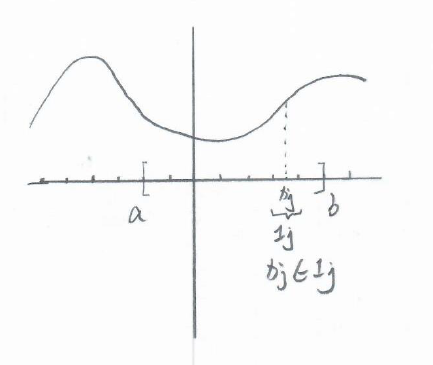
\includegraphics[width=0.3\linewidth,height=0.2\linewidth]{fig101.png}}
 	\label{img101}\qquad \qquad 
 	\subfloat[Lebesgue integration]{
 		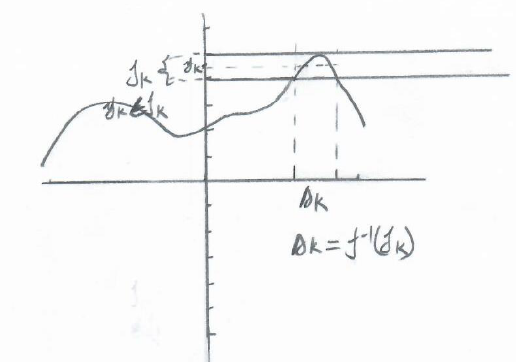
\includegraphics[width=0.3\linewidth,height=0.2\linewidth]{fig102.png}}
 	\label{img102}
 	\caption{Integration}
 \end{figure}

\begin{enumerate}
	\item Riemann integral
	\begin{equation}
	\int f  \approx \sum {f\left( {{x_j}} \right)} \left| {{I_j}} \right|
	\label{eq10.3}
	\end{equation}
	\item Lebesgue integration
	\begin{equation}
	I\left( f \right) \approx \sum {{y_k}\mu \left( {{A_k}} \right)}  = \sum\limits_k {{y_k}\mu \left( {{f^{ - 1}}\left( {{J_k}} \right)} \right)} 
	\end{equation}
	where ${A_k} = {f^{ - 1}}\left( {{J_k}} \right)$.
\end{enumerate}

In defining measurability we will want to consider functions
\begin{equation}
f:\Omega  \to \mathbb{R} \cup \left\{ { - \infty ,\infty } \right\} = \overline {\mathbb{R}}
\label{eq10.5}
\end{equation}
It is possible to define the class of Borel sets $\mathcal{B}$ in $ \overline {\mathbb{R}} $ in terms of this topology. However, we adopt the simple procedure of defining the class 
\begin{equation}
\overline {\mathcal{B}}  = \left\{ {A \cup B,A \in {\mathcal{B}},B \subseteq \left\{ { - \infty ,\infty } \right\}} \right\}
\label{eq10.6}
\end{equation}

\begin{proposition}
	$ \overline {\mathcal{B}} $ is a$ \sigma $-algebra.
\end{proposition}

\begin{definition}
	A function $f:\Omega  \to \overline {\mathbb{R}} $ is said to be $\mathcal{F}-$measurable if and only if 
	\begin{equation}
	{f^{ - 1}}\left( A \right) \in \mathcal{F}
	\end{equation}
	for all $A \in \overline {\mathcal{B}} $.
	\label{def10.1}
\end{definition}

If there is only one $\sigma-$field $\mathcal{F}$ under discussion we may say that $ f $ is a measurable function.

{\color{red} 
	\begin{remark}
		\begin{equation}
		\mathcal{F} \subseteq \mathcal{G}
		\end{equation}
	\end{remark}

}

\begin{lemma}
	$\left( {\Omega ,\mathcal{F},\mu } \right)\;f:\Omega  \to \overline {\mathbb{R}} $, $ f $ is measurable each of the following conditions is necessary and sufficient:
	\begin{enumerate}
		\item ${f^{ - 1}}\left( {\left( { - \infty ,x} \right]} \right) \in \mathcal{F},\;\forall x \in \mathbb{R},\; i.e. \; \left\{ {\omega  \in \Omega ,f\left( \omega  \right) \leqslant x} \right\} \in \mathcal{F} $
		\item ${f^{ - 1}}\left( {\left( { - \infty ,x} \right)} \right) \in \mathcal{F},\;\forall x \in \mathbb{R},\; i.e. \; \left\{ {\omega  \in \Omega ,f\left( \omega  \right) < x} \right\} \in \mathcal{F}$
		\item ${f^{ - 1}}\left( \left[ {x,\infty } \right) \right) \in \mathcal{F},\;\forall x \in \mathbb{R},\; \;  i.e. \; \left\{ {\omega  \in \Omega ,f\left( \omega  \right) \ge x} \right\} \in \mathcal{F} $
		\item ${f^{ - 1}}\left( {\left( { x, \infty} \right)} \right) \in \mathcal{F},\;\forall x \in \mathbb{R},\; \; i.e. \; \left\{ {\omega  \in \Omega ,f\left( \omega  \right) > x} \right\} \in \mathcal{F}$
	\end{enumerate}
\label{lma10.1}
\end{lemma}

\begin{proof}
	We only proof (1) in Lemma \ref{lma10.1} 
	\begin{enumerate}
		\item $ \Rightarrow $ $ \left( { - \infty ,x} \right] \in \overline {\mathcal{B}} $ 
		\item $ \Leftarrow $ If we suppose that the condition is satisfied, and put
		\begin{equation}
		\mathcal{C} = \left\{ {A \in \overline {\mathcal{B}} ,{f^{ - 1}}\left( A \right) \in {\mathcal{F}}} \right\}
		\label{eq10.9}
		\end{equation}
		then
		\begin{enumerate}
			\item $ \mathcal{C} $ is a $ \sigma $-algebra 
			\item $ \mathcal{C} \supseteq\mathcal{G} = \left\{ {\left( { - \infty ,x} \right],x \in \mathbb{R}} \right\} $
		\end{enumerate}
	by $ a\&b $ ,
	\begin{equation}
	\mathcal{C} \supseteq \mathcal{F}\left( \mathcal{G} \right) \supseteq \overline {\mathcal{B}} 
	\label{eq10.10}
	\end{equation}
	then $ \mathcal{C} $ is a $ \sigma $-algebra.
	\begin{itemize}
		\item $\overline {\mathbb{R}}  \in \mathcal{C},{f^{ - 1}}\left( {\overline {\mathbb{R}} } \right) = \left\{ {\omega  \in \Omega ,f\left( \omega  \right) \in \overline {\mathbb{R}} } \right\} = \Omega  \in {\mathcal{F}}$
		\item $ A \in \mathcal{C} \Rightarrow A^{c} \in \mathcal{C}, {f^{ - 1}}\left( A \right) \in \mathcal{F} $, so ${f^{ - 1}}\left( {{A^c}} \right) \in {f^{ - 1}}{\left( A \right)^c} \in \mathcal{F}$
		\item ${A_j} \in \mathcal{C} \Rightarrow \bigcup\limits_{j \geqslant 1} {{A_j}}  \in \mathcal{C}$, then
		\begin{equation}
		{f^{ - 1}}\left( {\bigcup\limits_{j \geqslant 1} {{A_j}} } \right) = \bigcup\limits_j {\;\underbrace {{f^{ - 1}}\left( {{A_j}} \right)}_{ \in {\mathcal{F}}}}  \in {\mathcal{F}}
		\label{eq10.11}
		\end{equation}
	\end{itemize}	
	\end{enumerate}
%	\begin{enumerate}
%		\setcounter{enumi}{5}
%		\item $ \mathcal{C} $ is a $ \sigma $-algebra 
%		\item $ \mathcal{C} \supseteq\mathcal{G} = \left\{ {\left( { - \infty ,x} \right],x \in \mathbb{R}} \right\} $
%    \end{enumerate}
\end{proof}

Given $\left( {\Omega ,\mathcal{F},\mu } \right)$ as above. If $\Omega  = \bigcup\limits_{i = 1}^n {{E_i}} $ and the sets $ E_{i} $ are disjoint (${E_j} \cap {E_k} = \emptyset ,\;j \ne k$), then $ E_{1},E_{2},...,E_{n} $ are said to form a (finite) dissection of $ \Omega $. They are said to form an $ \mathcal{C} $-dissection if, in addition $ E_{i} \in \mathcal{F}(i=1,2,...,n) $.

\begin{definition}[Simple Function]
	A function $f:\;\Omega  \to \mathbb{R}$ is called $ \mathcal{F} $-simple if it can be expressed as
	\begin{equation}
	f = \sum\limits_{j = 1}^n {{c_j}\;{1_{{E_j}}}} ,\;{c_j} \in \mathbb{R}
	\label{eq10.12}
	\end{equation}
	where $ 1_{E_{j}}, \Omega  \to \overline {\mathbb{R}}$,
	\begin{equation}
	\omega  \mapsto {1_{{E_j}}}\left( \omega  \right) = \left\{ {\begin{matrix}
		{1,}  \\ 
		{0,}  \\ 
		
		\end{matrix} } \right.\;\begin{matrix}
	{\omega  \in {E_j}}  \\ 
	{\omega  \notin {E_j}}  \\ 
	
	\end{matrix}
	\label{eq10.13} 
	\end{equation}
	\label{def10.2}
	and $\sum\limits_{j = 1}^n {{E_j}}  = \Omega ,\;{E_0} = \Omega \backslash \left( {\sum\limits_{j = 1}^n {{E_j}} } \right) \in \mathcal{F}$.
\end{definition}

If there is only one $\sigma-$field $\mathcal{F}$ under discussion we will talk of simple function rather than $ \mathcal{F} $-simple functions.

${f^{ - 1}}\left( A \right) = \sum\limits_{k,{c_k}} {{E_k}}  \in {\mathcal{F}},\;A \in \overline {\mathcal{B}},$ $f:\Omega  \to R{}_ + ,\;f = \sum\limits_{j = 1}^n {{c_j}{1_{{E_j}}}} ,\;{E_j} \in {\mathcal{F}},\;\left\{ {{E_1},...,{E_n}} \right\}\;partition\;of\;\Omega $.

\begin{figure}[!htb]
	\centering
	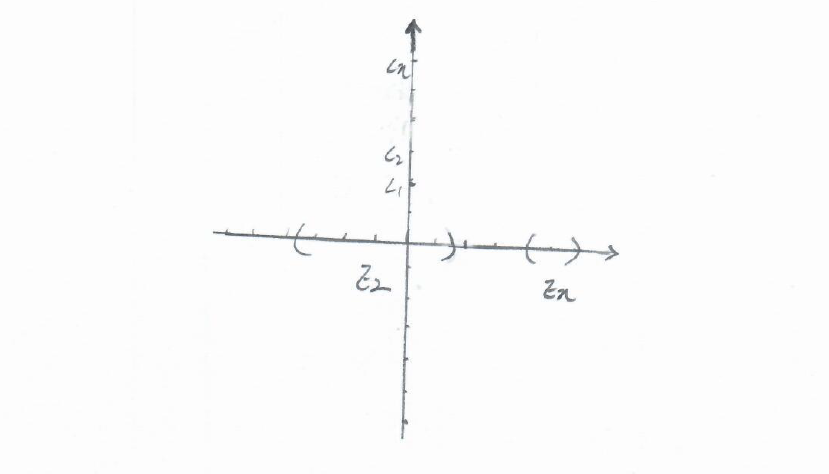
\includegraphics[width=0.6\linewidth,height=0.2\linewidth]{/fig103.png}
	%\caption{Unfolding of recurrency}
\end{figure}

\begin{equation}
I\left( f \right) = \sum\limits_{j = 1}^n {{c_j}\mu \left( {{E_j}} \right)} 
\label{eq10.14}
\end{equation}
where ${c_j} \geqslant 0$.

If $f = \sum\limits_{k = 1}^m {{d_k}{1_{{F_k}}}} $.

\begin{proposition}
	${E_{{j^ \circ }}} \cap {F_{{k^ \circ }}} \ne \emptyset $, then 
	\begin{equation}
	\sum\limits_{j = 1}^n {{c_j}\mu \left( {{E_j}} \right)}  = \sum\limits_{k = 1}^n {{d_k}\mu \left( {{F_k}} \right)} 
	\end{equation}
	\label{prop10.2}
\end{proposition}

\begin{proof}
	\begin{equation}
	\begin{split}
	\mu \left( {{E_j}} \right) & = \mu \left( {{E_j} \cap \left( {\sum\limits_{k = 1}^m {{F_k}} } \right)} \right)\\
							   & = \mu \left( {\sum\limits_{k = 1}^m {{{\left( {{E_j} \cap F_{k}} \right)}}} } \right)\\
							   & = \mu \left( {{E_j}} \right) = \sum\limits_{k = 1}^m {\mu \left( {{E_j} \cap {F_k}} \right)}
	\end{split}
	\label{eq10.16}
	\end{equation}
	then
	\begin{equation}
	\begin{split}
	\sum\limits_{j = 1}^n {{c_j}\mu \left( {{E_j}} \right)} & = \sum\limits_{j = 1}^n {\sum\limits_{k = 1}^m {{c_j}\mu \left( {{E_j} \cap {F_k}} \right)} } \\
															&  = \sum\limits_{j = 1}^n {\sum\limits_{k = 1}^m {{d_k}\mu \left( {{E_j} \cap {F_k}} \right)} } \\
															& = \sum\limits_{k = 1}^m {{d_k}\mu \left( {{F_k}} \right)} 
	\end{split}
	\end{equation}
\end{proof}

\begin{proposition}
	\text{}
	\begin{enumerate}
		\item $f:\;\Omega  \to {\overline {\mathbb{R}} _ + }$ measurable then there exists ${\left( {{f_n}} \right)_{n \geqslant 1}},\;{f_n}$ simple functions, such that ${f_n} \geqslant 0,\;{f_n} \uparrow f$
		\item $I\left( f \right) = \mathop {\lim }\limits_n \;I\left( {{f_n}} \right)$
		\item $f:\;\Omega  \to \overline {\mathbb{R}} $ measurable, ${f^ + } = \max \left( {f,0} \right),\;{f^ - } = \max \left( { - f,0} \right),\;{f^ + },{f^ - }$ measurable then $f = {f^ + } - {f^ - }$, then 
		\begin{equation}
		I\left( f \right) = I\left( {{f^ + }} \right) - I\left( {{f^ - }} \right)
		\label{eq10.18}
		\end{equation}
	\end{enumerate}
	\label{prop10.3}
\end{proposition}

\begin{example}
	$\Omega  = \left( {0,1} \right],\;{\mathcal{B}},\lambda ,\;\;E = \mathbb{Q} \cap \Omega ,\;f = {1_{{E^c}}}\;$, i.e.  $ f $ simple, then
	\begin{equation}
	I\left( f \right) = \lambda \left( {{E^c}} \right) = 1
	\label{eq10.19}
	\end{equation} 
\end{example} 
%\classheader{Lecture 11}
\setcounter{lecture}{11}
\begin{center}
	\Large \bf Measurable Functions
\end{center}
\vspace{0.25cm}

We now assume given $\left( {\Omega ,\mathcal{F},\mu } \right)$, where $ \Omega $ is a space, $ \mathcal{F} $ a $ \sigma $-field of subsets of $ \Omega $ and $ \mu $ a measure on $ \mathcal{F} $.

 \begin{lemma}
 	If $ f $ and $ g $ are measurable functions: $\Omega  \to \overline {\mathbb{R}} $, and $ \alpha \in \mathbb{R} $, then
 	\begin{enumerate}
 		\item $ \alpha f \in \mathcal{F} $-measurable
 		\item $ \alpha + f  $ $\in \mathcal{F} $-measurable
 		\item $ f + g \in \mathcal{F} $-measurable
 		\item $f^{2} \in \mathcal{F} $-measurable
 		\item ${1 \mathord{\left/
 				{\vphantom {1 f}} \right.
 				\kern-\nulldelimiterspace} f}\in \mathcal{F} $-measurable
 		\item $ f^{+},f^{-} $, $\left| f \right| \in \mathcal{F} $-measurable
 		\item $ fg \in \mathcal{F} $-measurable
 	\end{enumerate}
 \label{lma11.1}
 \end{lemma}
\begin{proof}
	\text{}
	\begin{enumerate}
		\item $ \alpha f \in \mathcal{F} $-measurable, we want to show that $\left\{ {\omega :\alpha f\left( \omega  \right) \leqslant x} \right\} \in \mathcal{F}$
		\begin{enumerate}
			\item $ \alpha = 0 $
			\item $ \alpha > 0 $, $\alpha f\left( \omega  \right) \leqslant x,\;i.e.\;f\left( \omega  \right) \leqslant {\raise0.7ex\hbox{$x$} \!\mathord{\left/
					{\vphantom {x \alpha }}\right.\kern-\nulldelimiterspace}
				\!\lower0.7ex\hbox{$\alpha $}}\;by\;\left\{ {\omega :\;f\left( \omega  \right) \leqslant {\raise0.7ex\hbox{$x$} \!\mathord{\left/
						{\vphantom {x \alpha }}\right.\kern-\nulldelimiterspace}
					\!\lower0.7ex\hbox{$\alpha $}}} \right\} \in \;\mathcal{F},\;\forall \ {\raise0.7ex\hbox{$x$} \!\mathord{\left/
					{\vphantom {x \alpha }}\right.\kern-\nulldelimiterspace}
				\!\lower0.7ex\hbox{$\alpha $}} \in \mathbb{R}$
			\item $ \alpha < 0 $,  $\alpha f\left( \omega  \right) \leqslant x,\;i.e.\;f\left( \omega  \right) \geqslant {\raise0.7ex\hbox{$x$} \!\mathord{\left/
					{\vphantom {x \alpha }}\right.\kern-\nulldelimiterspace}
				\!\lower0.7ex\hbox{$\alpha $}}\;\;$ then by lemma \ref{lma10.1}. 
		\end{enumerate}
		\item 
		\item  we want to show $f + g\; \in \mathcal{F}$-measurable, i.e. $\left\{ {\omega :f\left( \omega  \right) + g\left( \omega  \right) < x} \right\} \in \mathcal{F},\;\forall x \in \mathbb{R}$
		
		\begin{equation}
		\left\{ {\omega :f\left( \omega  \right) + g\left( \omega  \right) < x} \right\} = \bigcup\limits_{r \in \mathbb{Q}} {\left( {\left\{ {\omega :f\left( \omega  \right) < r} \right\} \cap \left\{ {g\left( \omega  \right) < x - r} \right\}} \right)} 
		\label{eq11.1}
		\end{equation}
		
		by Lemma \ref{lma10.1}, and $ \mathcal{F} $ is a $ \sigma $-algebra, so $\left\{ {\omega :f\left( \omega  \right) + g\left( \omega  \right) < x} \right\} \in \mathcal{F}$
		\item $ f^{2} \in \mathcal{F} $-measurable
		
		Now, we will check $\left\{ {\omega :f{{\left( \omega  \right)}^2} < x} \right\} \in \mathcal{F}$
		
		\begin{equation}
		\left\{ {\omega :f{{\left( \omega  \right)}^2} < x} \right\} = \left\{ {\begin{matrix}
			{\emptyset  \in \mathcal{F}}  \\ 
			{\left\{ {\omega  \in \Omega , - x < f\left( \omega  \right) < x} \right\} \in \mathcal{F}}  \\ 
			
			\end{matrix} } \right.\;\;\;\begin{matrix}
		{x \leqslant 0}  \\ 
		{x > 0}  \\ 
		
		\end{matrix} 
		\label{eq11.2}
		\end{equation}
		\item $\frac{1}{f} \in \mathcal{F}$-measurable i.e. $\left\{ {\omega  \in \Omega :\frac{1}{{f\left( \omega  \right)}} < x} \right\} \in \mathcal{F}$
		
		by 
		\begin{enumerate}
			\item $ x > 0 $, $\left\{ {\omega :f\left( \omega  \right) < 0} \right\} \cup \left\{ {\omega :f\left( \omega  \right) > \frac{1}{x}} \right\} \in \mathcal{F}$
			\item $ x = 0 $, $\left\{ {\omega :f\left( \omega  \right) < 0} \right\} \in \mathcal{F}$
			\item $ x < 0 $, $\left\{ {\omega :\frac{1}{x} < f\left( \omega  \right) < 0} \right\} \in \mathcal{F}$
		\end{enumerate}
		\item ${f^ + } = \max \left\{ {f,0} \right\}$
		\begin{equation}
		\left\{ {\omega  \in \Omega :{f^ + }\left( \omega  \right) < x} \right\} = \left\{ {\begin{matrix}
			{\emptyset  \in \mathcal{F}}  \\ 
			{\left\{ {\omega  \in \Omega :f\left( \omega  \right) < x} \right\} \in \mathcal{F}}  \\ 
			
			\end{matrix} } \right.\;\;\;\begin{matrix}
		{x \leqslant 0}  \\ 
		{x > 0}  \\ 
		
		\end{matrix} 
		\label{eq11.3}
		\end{equation}
		
		${f^ - } = \max \left( { - f,0} \right)$ and $\left| f \right| = {f^ + } + {f^ - }$
		\item by $fg = \frac{1}{2}\left( {{{\left( {f + g} \right)}^2} - {f^2} - {g^2}} \right)$
	\end{enumerate}
\end{proof}

\begin{remark}
	\begin{equation}
	\begin{split}
	\max \left( {f,g} \right) & = \frac{1}{2}\left[ {f + g + \left| {f - g} \right|} \right]\\
	\min \left( {f,g} \right) & = f + g - \max \left( {f,g} \right)
	\end{split}
	\label{eq11.4}
	\end{equation}
\end{remark}
%\classheader{Lecture 12}
\setcounter{lecture}{12}
\begin{center}
	\Large \bf Definition of The Integral
\end{center}
\vspace{0.25cm}
 

%\classheader{Lecture 13}
\setcounter{lecture}{13}
\begin{center}
	\Large \bf Integral of Simple Functions
\end{center}
\vspace{0.25cm}
 
 
%\classheader{Lecture 14}
\setcounter{lecture}{14}
\begin{center}
	\Large \bf Properties of The Integral I
\end{center}
\vspace{0.25cm}
 

%\classheader{Lecture 15}
\setcounter{lecture}{15}
\begin{center}
	\Large \bf Properties of The Integral II
\end{center}
\vspace{0.25cm}
 
 
%\classheader{Lecture 16}
\setcounter{lecture}{16}
\begin{center}
	\Large \bf Theorems on The Convergence of Integrals
\end{center}
\vspace{0.25cm}
 
 
%\classheader{Lecture 17}
\setcounter{lecture}{17}
\begin{center}
	\Large \bf Product Measures
\end{center}
\vspace{0.25cm}
 

%\classheader{Lecture 18}
\setcounter{lecture}{18}
\begin{center}
	\Large \bf Measure On a Countable Product of Spaces
\end{center}
\vspace{0.25cm}
 

%\classheader{Lecture 19}
\setcounter{lecture}{19}
\begin{center}
	\Large \bf Fubini's Theorem
\end{center}
\vspace{0.25cm}
 
 
%\classheader{Lecture 20}
\setcounter{lecture}{20}
\begin{center}
	\Large \bf Hahn-Jordan Theorem
\end{center}
\vspace{0.25cm}
 

%\classheader{Lecture 21}
\setcounter{lecture}{21}
\begin{center}
	\Large \bf Radon-Nikodym Theorem
\end{center}
\vspace{0.25cm}
 
 
%\classheader{Lecture 22}
\setcounter{lecture}{22}
\begin{center}
	\Large \bf Almost Sure and Almost Uniform
\end{center}
\vspace{0.25cm}
 
 
%\classheader{Lecture 23}
\setcounter{lecture}{23}
\begin{center}
	\Large \bf Convergence in Measure
\end{center}
\vspace{0.25cm}
 

%\classheader{Lecture 24}
\setcounter{lecture}{24}
\begin{center}
	\Large \bf H$\mathop o\limits^ {\cdot \cdot} $elder and Minkowski inequalities
\end{center}
\vspace{0.25cm}
 

%\classheader{Lecture 25}
\setcounter{lecture}{25}
\begin{center}
	\Large \bf $ L_{p} $ Spaces
\end{center}
\vspace{0.25cm}
 

%\classheader{Lecture 26}
\setcounter{lecture}{26}
\begin{center}
	\Large \bf From Convergence in Measure to Convergence in $ L_{p} $
\end{center}
\vspace{0.25cm}
 

%\classheader{Lecture 27}
\setcounter{lecture}{27}
\begin{center}
	\Large \bf Bounded Linear Operators in  $ L_{p} $
\end{center}
\vspace{0.25cm}
 

%\classheader{Lecture 28}
\setcounter{lecture}{28}
\begin{center}
	\Large \bf Vitali's Covering Lemma
\end{center}
\vspace{0.25cm}
 

%\classheader{Lecture 29}
\setcounter{lecture}{29}
\begin{center}
	\Large \bf  Differentiability of Functions of Bounded Variations
\end{center}
\vspace{0.25cm}
 

%\classheader{Lecture 30}
\setcounter{lecture}{30}
\begin{center}
	\Large \bf  Absolutely Continuous Functions
\end{center}
\vspace{0.25cm}
 

%\classheader{Lecture 31}
\setcounter{lecture}{31}
\begin{center}
	\Large \bf  Decomposition of Distribution
\end{center}
\vspace{0.25cm}
 

%\classheader{Lecture 32}
\setcounter{lecture}{32}
\begin{center}
	\Large \bf  Cantor Ternary Set and Function
\end{center}
\vspace{0.25cm}
 



\end{document}
